\noindent\enquote{\itshape Not many people have a timber forest of their own.  }\bigbreak

\hfill Lars Mytting - Norwegian Wood 

\vspace*{0.05\textheight}

In this chapter we shall exhaustively, yet briefly, describe the specific numerical methods used throughout this thesis. Providing the necessary detail to contextualise the results presented in the subsequent chapters. This will not be an exhaustive introduction to any of the presented methods, as these topics could and indeed do span multiple books and articles. Rather, we shall be presenting the implementations of each given method as it manifests results in the following work - placing each implementation within the context of the broader literature regarding these methods. We shall be presenting the following methods: the Greens Dydaic Method for determining meso-scale light-matter interactions; classical molecular dynamics for computing structural and thermodynamic properties of nanoalloys; and density functional theory as an \textit{ab initio} method for evaluating systems whose dynamics and properties are fundamentally quantum mechanical in nature.

\section{Greens Dyadic Method}
\label{sec:GDM}
For a fast evaluation and screening of the extinction spectrum of the breathing cages, we have also chosen to adopt a classical approach via the Green's Dyadic Method (GDM) \cite{GDM,Girard_2005},  as implemented in the pyGDM code \cite{pyGDM,pyGDMarXiv}. This method approximates each atom to be a dipole oscillator existing within the coupled dipole approximation. This method neglects explicit electron contributions, hence correlated behaviour that may arise from quantum many-body effects. However, this particular implementation has the benefit of considering the exact position of each atom - respecting the desired geometry of the system whilst maintaining the relative computational simplicity of a classical approach. An additional advantage of the pyGDM realisation of the GDM method is that, in contrast to most other coupled-dipole codes, pyGDM uses a generalised propagator, which hugely boosts the performance when solving large monochromatic problems.
In brief, the GDM seeks to resolve an optical Lippmann-Schwinger equation, calculating the total electromagnetic field inside a nanostructure embedded in a fixed environment. Such systems do not require the presence of an external field, indeed the Lippmann-Schwinger equation self-consistently relates the zero-order field and the total field upon interaction. However, we have elected to illuminate our structures with a series of monochromatic plane waves within the considered spectral range.
%
To evaluate the extinction spectrum, we need only consider the interaction of the dipole moment and total field in each discretised volume cell as,
\begin{equation}
    \sigma_{ext}\left( \omega \right) = \frac{8\pi^{2}}{n_{env}\lambda_{0}} \sum_{j}^{N_{cells}} \Im \left( \textbf{E}_{0,j} \cdot \textbf{P}_{j} \right),
    \label{eqn:ext_gdm}
\end{equation}
wherein $n_{env}$, $\lambda_{0}$, and $\textbf{P}_{j}$ are respectively the dielectric constant of the embedding environment, the incident wavelength, the dipole moment of cell $j$, and $E_{0,j}=E_0(r_j)$ is the incident field \cite{Dipole_Spec_Class}. In the described method, the near field may be found by self-consistently solving
\begin{equation}
    \textbf{E} \left( \textbf{r}_{i}, \omega \right) = \textbf{E}_{0} \left( \textbf{r}_{i}, \omega \right) + \sum_{j}^{N_{Cells}} G_{tot}^{EE} \left( \textbf{r}_{i},\textbf{r}_{j}, \omega \right) \chi \textbf{E}'\left( \textbf{r}_{j}, \omega \right) V_{cell},
    \label{eqn:GDM}
\end{equation}
which is essentially a Lippmann-Schwinger equation where $G_{tot}^{EE} \left( \textbf{r}_{i},\textbf{r}_{j}, \omega \right)$ is the Green's dyad to be solved, $\chi$ is the metal's susceptibility, and $V_{cell}$ is the volume of a unit cell. From this field, we then calculate the effective dipole moments, $\mathbf{P}_j= V_{cell} \chi_j \cdot \mathbf{E}_j$, from the internal field distribution.

Equation \ref{eqn:GDM} provides a self consistent relationship between the local fields $\textbf{E} \left( \textbf{r}_{i}, \omega \right)$, and the illumination fields, $\textbf{E}_{0} \left( \textbf{r}_{i}, \omega \right)$ for the internal mesh point $i$ within the structure. In general, one should also consider the magnetic Green's dyad, and moreover, the mixed field susceptibilities described by $G_{tot}^{EH} \left( \textbf{r}_{i},\textbf{r}_{j}, \omega \right)$, and $G_{tot}^{HE} \left( \textbf{r}_{i},\textbf{r}_{j}, \omega \right)$. These propagators are treated in precisely the same fashion outlined in Equation \ref{eqn:GDM}, and so we shall not explicitly write them down.

In reality, very few materials interact strongly with the magnetic component of an electromagnetic wave, the given implementation of the method has omitted the consideration of the $G_{tot}^{HH} \left( \textbf{r}_{i},\textbf{r}_{j}, \omega \right)$ contribution to the 6$\times$6 super-propagator $\mathbb{G}$ whose components are the previously described Green's dyads.

With knowledge of the functional form of the incident field, and a sufficiently converged internal field distribution, one is able to compute the extinction spectrum for a given finite system held within a dispersive medium, as described by Equation \ref{eqn:ext_gdm}. The described methodology is simply a maturation of the generalised field propagators for electromagnetic scattering described in \cite{PhysRevLett.74.526}. All metallic dielectric parameters used in these calculations are provided by Johnson and Christie \cite{PhysRevB.6.4370}.

To introduce this given method to an atomistic consideration, we have chosen to set the mesh points to be the atomic coordinates of a nanoparticle where these given mesh points may inherit the dielectric properties of the given material. In doing so, we are able to exercise a high degree of control over the morphology of the scattering structure through the creation of the grid points. Moreover, given that the field susceptibilities in Equation \ref{eqn:GDM} are described by the aforementioned dielectric functions of a specified material, one may arbitrarily choose to use alternative data sets to better describe disparate structural conformations. A further point to make is that it is possible to compute these material properties using \textit{ab initio} techniques. Therefore, this model may in equal measure utilise experimental data or \textit{ab initio} data to make predictions at the nanoscale.

A consequence of using known dielectric constants explicitly extracted from systems whose physical size is far greater than that of our own clusters is that it is not unlikely that our systems may begin to appear translucent under illumination. As we are firmly within the quasi-static dipole approximation, by considering structures on the order of 1 nm and illuminating within the UV~-~vis~-~NIR (ultraviolet~-~visible~-~near~-~infrared), we may find that the incident field will only weakly couple to the structure and result in non-trivial internal field enhancement as a consequence of this translucency. This is indeed a limitation of the method, and should serve as a stark reminder of the necessity of an \textit{ab initio} method at the nanometric scale. Nonetheless, given the nature of the coupled dipole approximation relying on coulombic interactions, we may still utilise this method as a fast screening process to search for evidence of novel behaviour - even at such small size scales.


\section{Molecular dynamics}
\label{sec:CMD}
We now step into the classical domain, in that we wish to model the larger scale dynamics of the atoms themselves on timescales appropriate for the underlying physics. That is to say, we wish to observe dynamics which occur on timescales approaching microseconds. Whilst the timescales for observing the fluxional behaviour of NAs can be in the range of seconds to hours \cite{https://doi.org/10.1002/smll.201001138,https://doi.org/10.1002/smll.200801169}, it remains instructive to model and consider the timescales on which these processes may begin to occur to better understand the underlying dynamics and physics driving the experimentally observed behaviour. A characteristic example for nanoparticle synthesis is that of Ostwald ripening which has been shown to occur on the order of minutes to hours \cite{doi:10.1021/acs.langmuir.6b02662}.

While in principle, one can choose to include the electrons' contribution to the resultant forces acting upon individual ions, this is highly impracticable for systems larger than 1 nm. While such calculations are performed, it is rare to create trajectories longer than tens of picoseconds in length due to the high cost of solving considering explicitly the electron contributions at every time step. This is indeed true for systems $>$10 nm in size which contain thousands of atoms, and therefore tens of thousands of electrons. Suffice to say, if one wishes to observe events such as adsorption or diffusion on systems larger than a few nanometers, then one must be willing to compromise on the accuracy afforded by explicit quantum mechanical consideration. However; we find that this is indeed a sacrifice worth making as we are, in principle, able to model the dynamics of a cluster for a sufficient amount of time that we may observe a `rare event'. For example, the folding event of a protein which has been deformed from its native conformation. Moreover, we may collect statistics and sample the phase space with specific techniques. In general, there are two primary methods of exploring the phase space of a microscopic system. Either by explicit time dependent integration of Newton's equations, molecular dynamics; or by considering the thermodynamic properties of many configurations relative to one another, Monte Carlo methods. While we acknowledge the utility and success of the latter, we are primarily concerned with the former in this work.

Many algorithms have been proposed in the previous decades to project the physical state of a system through time, with one of the most successful being the Velocity-Verlet algorithm. At its core, this is simply the discretised integration of Newton's equations motion. This algorithm is time reversible and has an error scaling as $\mathcal{O}( \Delta t^{3} )$.

\begin{equation}
    r(t+\Delta t) = r(t) + v(t)\Delta t + \frac{F(t)} {2m}\left( \Delta t \right) ^{2} + \mathcal{O}{\Delta t^{3}}
    \label{eqn:vel-ver-r}
\end{equation}
\begin{equation}
    v(t+\Delta t) = v(t) + \frac{F(t) + F(t+\Delta t)}{2m}\left(\Delta t\right)^{2} + \mathcal{O}{\Delta t^{3}}
    \label{eqn:vel-ver-v}
\end{equation}



In the above equations, all symbols have their standard definition with respect to Newton's equations. However; it is worth acknowledging that there is not necessarily a specific requirement on what $\Delta t$ or $F(t)$ should be. In principle, the former should be set according to the phonon frequency of the system. Typically on the order of femtoseconds. This is to ensure that regions of phase space occupied by vibrational modes may be sufficiently and ergodically explored. In the case of the force, there is no single prescription on how the force acting on a given atom should be described. Recall that these forces are essentially the aggregation of Coulomb interactions between: ion - ion, electron - electron, ion - electron. The objective to describing interatomic interactions within a classical framework is to find a formulation for an effective model which may suitably describe the phenomena of interest, whilst neglecting features with negligible contributions or large computational overheads. We shall provide, below, the prescription used within the context of this research project.


\subsection{SMATB Potentials}
The modelling of large systems over long time scales is constrained by the trade-off between the accuracy and computational cost with respect to the modelling of interaction potentials between system components. In the case of nanoclusters, modelling atom-atom interactions within the second-moment of the tight-binding approximation is generally understood to be a reliable and efficient method. Two of the most common alternatives are the embedded atom model and the Rosato-Guillope-Legrande or Gupta (RGL) potentials \cite{RGL}, whose origins are within the second moment approximation of the tight binding model. Therefore, we shall heretoafter refer to this parameterisation as that of the SMATB. Given that we use only the SMATB potentials in our work, we shall limit our discussion here to the latter. 

It is known that the cohesive properties of transition metals, and their alloys, depend on the large $d$-band DoS with several thermodynamic and structural properties being largely insensitive to the finer details of the DoS, bur rather related to the average value and effective width \cite{refId0}. Describing the electronic DoS with respect to is moments is a tool to relate the electronic structure to the lattice since such moments are obtained by calculating products of matrix elements of the electronic Hamiltonian associated with closed paths of definite length. Each moment, $\mu_{k}$ may be interpreted as the contribution to the DoS coming from all possible closed electron paths of $k$ steps. In particular, the first moment, $\mu_{1}$ is related to the band centre energy, and fixes the energy scale. Experimentally, the binding energies of transition metals appear to be proportional to the average width of the DoS by $\sqrt{\mu_{2}}$ \cite{ALLAN1979142}. Within the tight binding (TB) model, subject to the constraint of local charge neutrality, an analytic expression for the first moments may be written if the sums are restricted to first neighbours only in FCC or HCP, and to second neighbours in BCC structures. Electron $d$-bands can subsequently be described by a basis of of two-centre integrals\footnote{Often described as \textit{hopping} or overlap integrals as the matrix elements describe the overlapping of the TB wave functions.} whose energy eigenvalues of the resultant matrix are classified, according to the magnetic quantum number of the basic orbitals, as $dd\sigma$, $dd\pi$, and $dd\delta$ - otherwise known as the Slater-Koster parameters\cite{PhysRev.94.1498}. Consequently, the moments then become linear combinations of these integrals. Indeed, one may proceed to express the second moment of the electronic DoS as a sum of squares of these hopping integrals as the following,

\begin{equation}
    \mu_{2} = z \left( dd\sigma^{2} + 2dd\pi^{2} + 2dd\delta^{2}\right),
    \label{eqn:mu2}
\end{equation}

 which describes matrix elements in the Hamiltonian with electron paths starting from a given site, hopping to another and returning to the original site, with $z$ being the coordination number.

These hopping integrals are a function of the radial distance between atoms $i$ and $j$ meaning that the binding energy, proportional to $\sqrt{mu_{2}}$, may be written for an atom $i$ as

\begin{equation}
    E_{i}^{B} = - \sqrt{ \sum_{j \in \lbrace neighbours \rbrace \neq i} \xi_{ab}^{2} e^{-2q_{ab}\left( \frac{r_{ij}}{r_{ab}^{0}} - 1 \right)} }
    \label{eqn:rgl_bind}
\end{equation}

with $r_{ij}$ being the separationd istance between atoms $i$ and $j$, $r_{ab}^{0}$ is defined by the bulk nearest-neighbour distance in the $ab$ lattice where $a$ and $b$ define the pairwise metals which may be considered to be interacting. $\xi$ is an effective hopping integral, and $q$ describes its dependence on the relative interatomic distance.

For the model to describe stable structures, a repulsive term is required which is given by a sum of Born~-~Mayer ion~-~ion repulsions,

\begin{equation}
    E_{i}^{R} = \sum_{j \in \lbrace neighbours \rbrace \neq i} A_{ab}e^{-p_{ab}\left( \frac{r_{ij}}{r_{ab}^{0}} - 1 \right) },
    \label{eqn:rgl_rep}
\end{equation}

whose origins may be considered to be from the increase in kinetic energy of conduction electrons constrained within two approaching ions \cite{ALLAN1979142}. In this instance, the parameter $p$ may be considered to be representative of the compressibility of the bulk material. Finally, $A_{ab}$, similarly to $\xi_{ab}$ in Equation \ref{eqn:rgl_bind}, is essentially a free parameter but is readily interpretable with respect to bulk material properties derived from the TB model.

Combining both the binding and repulsive terms fro Equations \ref{eqn:rgl_bind} and \ref{eqn:rgl_rep} respectively, one arrives at the full form for the SMATB potential as

\begin{equation}
    E_{RGL}^{i} = \sum_{j \in \lbrace neighbours \rbrace \neq i} A_{ab}e^{-p_{ab}\left( \frac{r_{ij}}{r_{ab}^{0}} - 1 \right) } - \sqrt{ \sum_{j \in \lbrace neighbours \rbrace \neq i} \xi_{ab}^{2} e^{-2q_{ab}\left( \frac{r_{ij}}{r_{ab}^{0}} - 1 \right)} }.
    \label{eqn:rgl}
\end{equation}

SMATB potentials depend on the set of all atomic coordinates and pairwise displacement vectors, $\textbf{r}_{ij}$, with the full potential being described by the sum over all atomic contributions.

It is worth noting that Equation \ref{eqn:rgl} is indeed heavily paramterised. However; many of these are easily recoverable from experiments and require little tuning. For example, the free parameters, $A_{ab}$, $\xi_{ab}$, $p_{ab}$, $q_{ab}$, and $r_{ab}^{0}$ are extracted from experimentally obtained values of cohesive energy, lattice parameters, and independent elastic constants for each system in the appropriate crystalline structure at $T=0$ $K$ under equilibrium conditions into consideration. The above expression describes the potential energy experienced by atom $i$ due to interactions with its neighbours. The most difficult parameter to set is the effective range of the potential, set by $r_{ab}$ in Equation \ref{eqn:rgl}, as this is, in effect, infinite and there may very well be strong long-range correlations. Nonetheless, we implement a cutoff which will typically be set to exist at approximately the second nearest neighbour distance, as observed in the bulk. In full consideration of Equation \ref{eqn:rgl}, we may state that $A_{ab}$, and $\xi_{ab}$ are derived from cohesive energies, $r_{ab}^{0}$ is defined by the bulk nearest-neighbour distance. Finally, $p_{ab}$, and $q_{ab}$ set the stiffness of the springs on which the potential is essentially coupling the atoms. Note that the indices $a$, $b$ define the pairwise metals which may be considered to be interacting. While it is possible to have trimetallic or even more complex systems modelled faithfully by Gupta potentials, one should note that by being an intrinsically two-body interaction, the number of required potential interactions would necessarily grow as a factorial.

The SMATB potential consists of an attractive and repulsive term. The repulsive component is modelled on the Born-Meyer term. The latter, attractive component is derived according to the second moment approximation of the tight binding, hence the naming convention. One considers the local density of states of electrons centred at a specific site and on a certain orbital; the resultant Hamiltonian of the system is given by an atomic level orbital contribution and by a hopping integral. By approximating the local density of states to be rectangular, consistent with the tight binding approximation, the attractive term may be recovered. We note that this approximation is well suited to transition metals given the strong $d$ character of their valence states. 

While it is true that many of these parameters may be recovered from experiment, one may also provide the parameters for more complex configurations from ab initio calculations. This may be especially useful in the case of highly mixed / alloyed structures in which a bulk like description is far from the simulated reality. Transferability to low dimensional cases has been established and validation of the parametrisation is done with respect to both static and dynamic quantities such as the energetic ranking of known geometries of a set of conformational isomers or the calculation of melting points. For bimetallic systems, the average of the monometallic parameters is usually sufficient to model hetero-metallic interactions. Especially in well separated systems where charge transfer effects are less significant. Gupta-like potentials are generally accurate for modestly sized systems (tens of atoms) and larger. Smaller than this and quantum mechanical finite size effects begin to become significant and electronic structure calculations are required to ensure fidelity. Fortunately, electronic calculations at this scale are relatively inexpensive.


\begin{table}[ht]
\centering
\caption{Parameters used for the computation of inter-atomic potentials used within the SMATB formalism.}
\label{tab:RGL}
\begin{tabular}{@{}lllllll@{}}
\toprule
Interaction & p & q & A (eV) & $\xi$ (eV)  & r$_{ab}^{0}$=$\sqrt{2}$r$_{0}$ (\AA) & Source      \\
\hline
Ag - Ag     & 10.928 & 3.139 & 0.1028 & 1.178 & 4.09 &  \cite{doi:10.1021/acs.jpcc.5b03577}  \\
Au - Au     & 10.229 & 4.036 & 0.2061 & 1.790 & 3.92 &  \cite{doi:10.1021/acs.jpcc.5b03577} \\
Cu - Cu     & 10.55 & 2.43 & 0.0894 & 1.2799 & 3.62 & \cite{CuPt}  \\
Pd - Pd     & 11.00 & 3.794 & 0.1715 & 1.7019 & 3.89 &  \cite{RGL_Pot}  \\
Pt - Pt     & 10.612 & 4.004 & 0.2975 & 2.695 & 3.92 & \cite{CuPt}  \\
%
Ag - Au     & 10.579 & 3.5875 & 0.15445 & 1.484 & 4.06 & \cite{doi:10.1021/acs.jpcc.5b03577}  \\
Ag - Cu     & 11.05 & 3.047 & 0.1539 & 1.5605 & 3.97 & \cite{PhysRevB.66.155420}   \\
Ag - Pd     & 10.895 & 3.492 & 0.161 & 1.5597 & 3.99 & \cite{doi:10.1063/1.1898223}   \\
Ag - Pt     & 10.73  & 3.57  & 0.175 & 1.79   & 4.00 & \cite{doi:10.1063/1.2897435}  \\
%
Au - Cu     & 11.05 & 3.047 & 0.1539 & 1.561 & 4.00 &  \cite{doi:10.1063/1.1898223} \\
Au - Pd     & 10.569 & 3.913 & 0.1843 & 2.082 & 3.99 & \cite{doi:10.1063/1.2897435}   \\
Au - Pt     & 10.42 & 4.02 & 0.250 & 2.20 & 3.97 &  \cite{doi:10.1098/rspa.2010.0562} \\
%
Cu - Pt     & 10.786 & 3.141 & 0.16 & 1.82 & 3.89 & \cite{CuPt}  \\
\bottomrule
\end{tabular}
\end{table}

We provide in Table \ref{tab:RGL}, the parameters used within the context of the following work. Each symbol has the same meaning outlined in Equation \ref{eqn:rgl}, and we have provided the originating source document for each of the specific interactions modelled. 

%%%%%%%%%%%%%%%%%%%%%%%%%%%%%%%%%%%%%%%%%%%%%%%%%%%%%%%%%%%%%%%%%%%%%%%%%%%%%%%%%
%%%%%%%%%%%%%%%%%%%%%%%%%%%%%%%%%%%%%%%%%%%%%%%%%%%%%%%%%%%%%%%%%%%%%%%%%%%%%%%%%

\subsection{Thermostats}

With the positions and velocities of all of the atoms updated according to the Velocity-Verlet equations, one is able to approximate the thermodynamic temperature of the system via the equipartition theorem, $\langle E_{kin}\rangle \propto 3K_{B}T$. In the case of simulating an isolated system evolving under its own dynamics, this is where the story may end. However; in the case of the canonical ensemble (NVT), one may wish to couple the system to a thermal reservoir to fix the temperature. As is the case with the selection of force field, the simulation of a thermal reservoir is a topic of active discussion within the community \cite{doi:10.1063/1.4792202,doi:10.1080/08927022.2021.1907382,Hu_2022,KE2022120116}. 

Exclusively used throughout the following work is the Anderson thermostat \cite{doi:10.1063/1.439486,doi:10.1063/1.2198824}. A characteristic timescale, $\tau$, for the thermostat is set for the system. A collision is then simulated according to a Poisson distribution with mean time between collisions set by $\tau$. This collision is modelled to be elastic as it rescales the velocity of a single atom from a Maxwell distribution set at the desired temperature. Given the types of system we are modelling, this is often not an inaccurate image we wish to capture. One should note that this thermostat requires the setting of the temperature for the Maxwell distribution and characteristic timescale for the collisions. Rare collisions will often result in slow convergence to a desired temperature whereas frequent collisions risks undersampling energetically prohibitive regions of the phase space. Indeed, it is this latter parameter which is so difficult to tune. Typically, it will be given as a frequency of order 100 GHz.

\begin{figure}
\centering
\begin{subfigure}[b]{0.45\textwidth}
    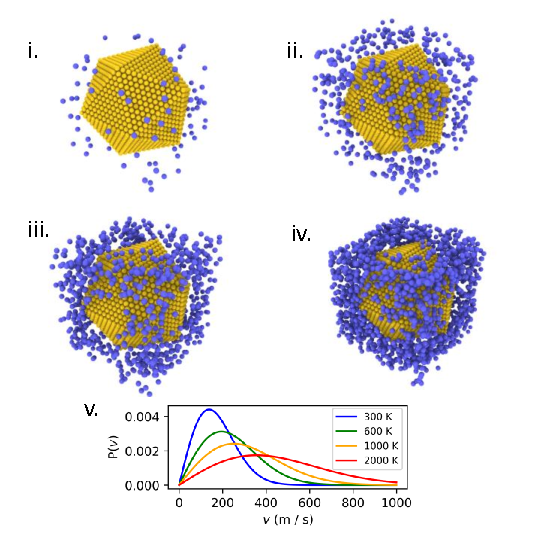
\includegraphics[width=\textwidth]{figures/Theory/Thermo.pdf}
    \caption{Andersen thermostat.} 
    \label{Fig:thermostat}
\end{subfigure}
\begin{subfigure}[b]{0.5\textwidth}
    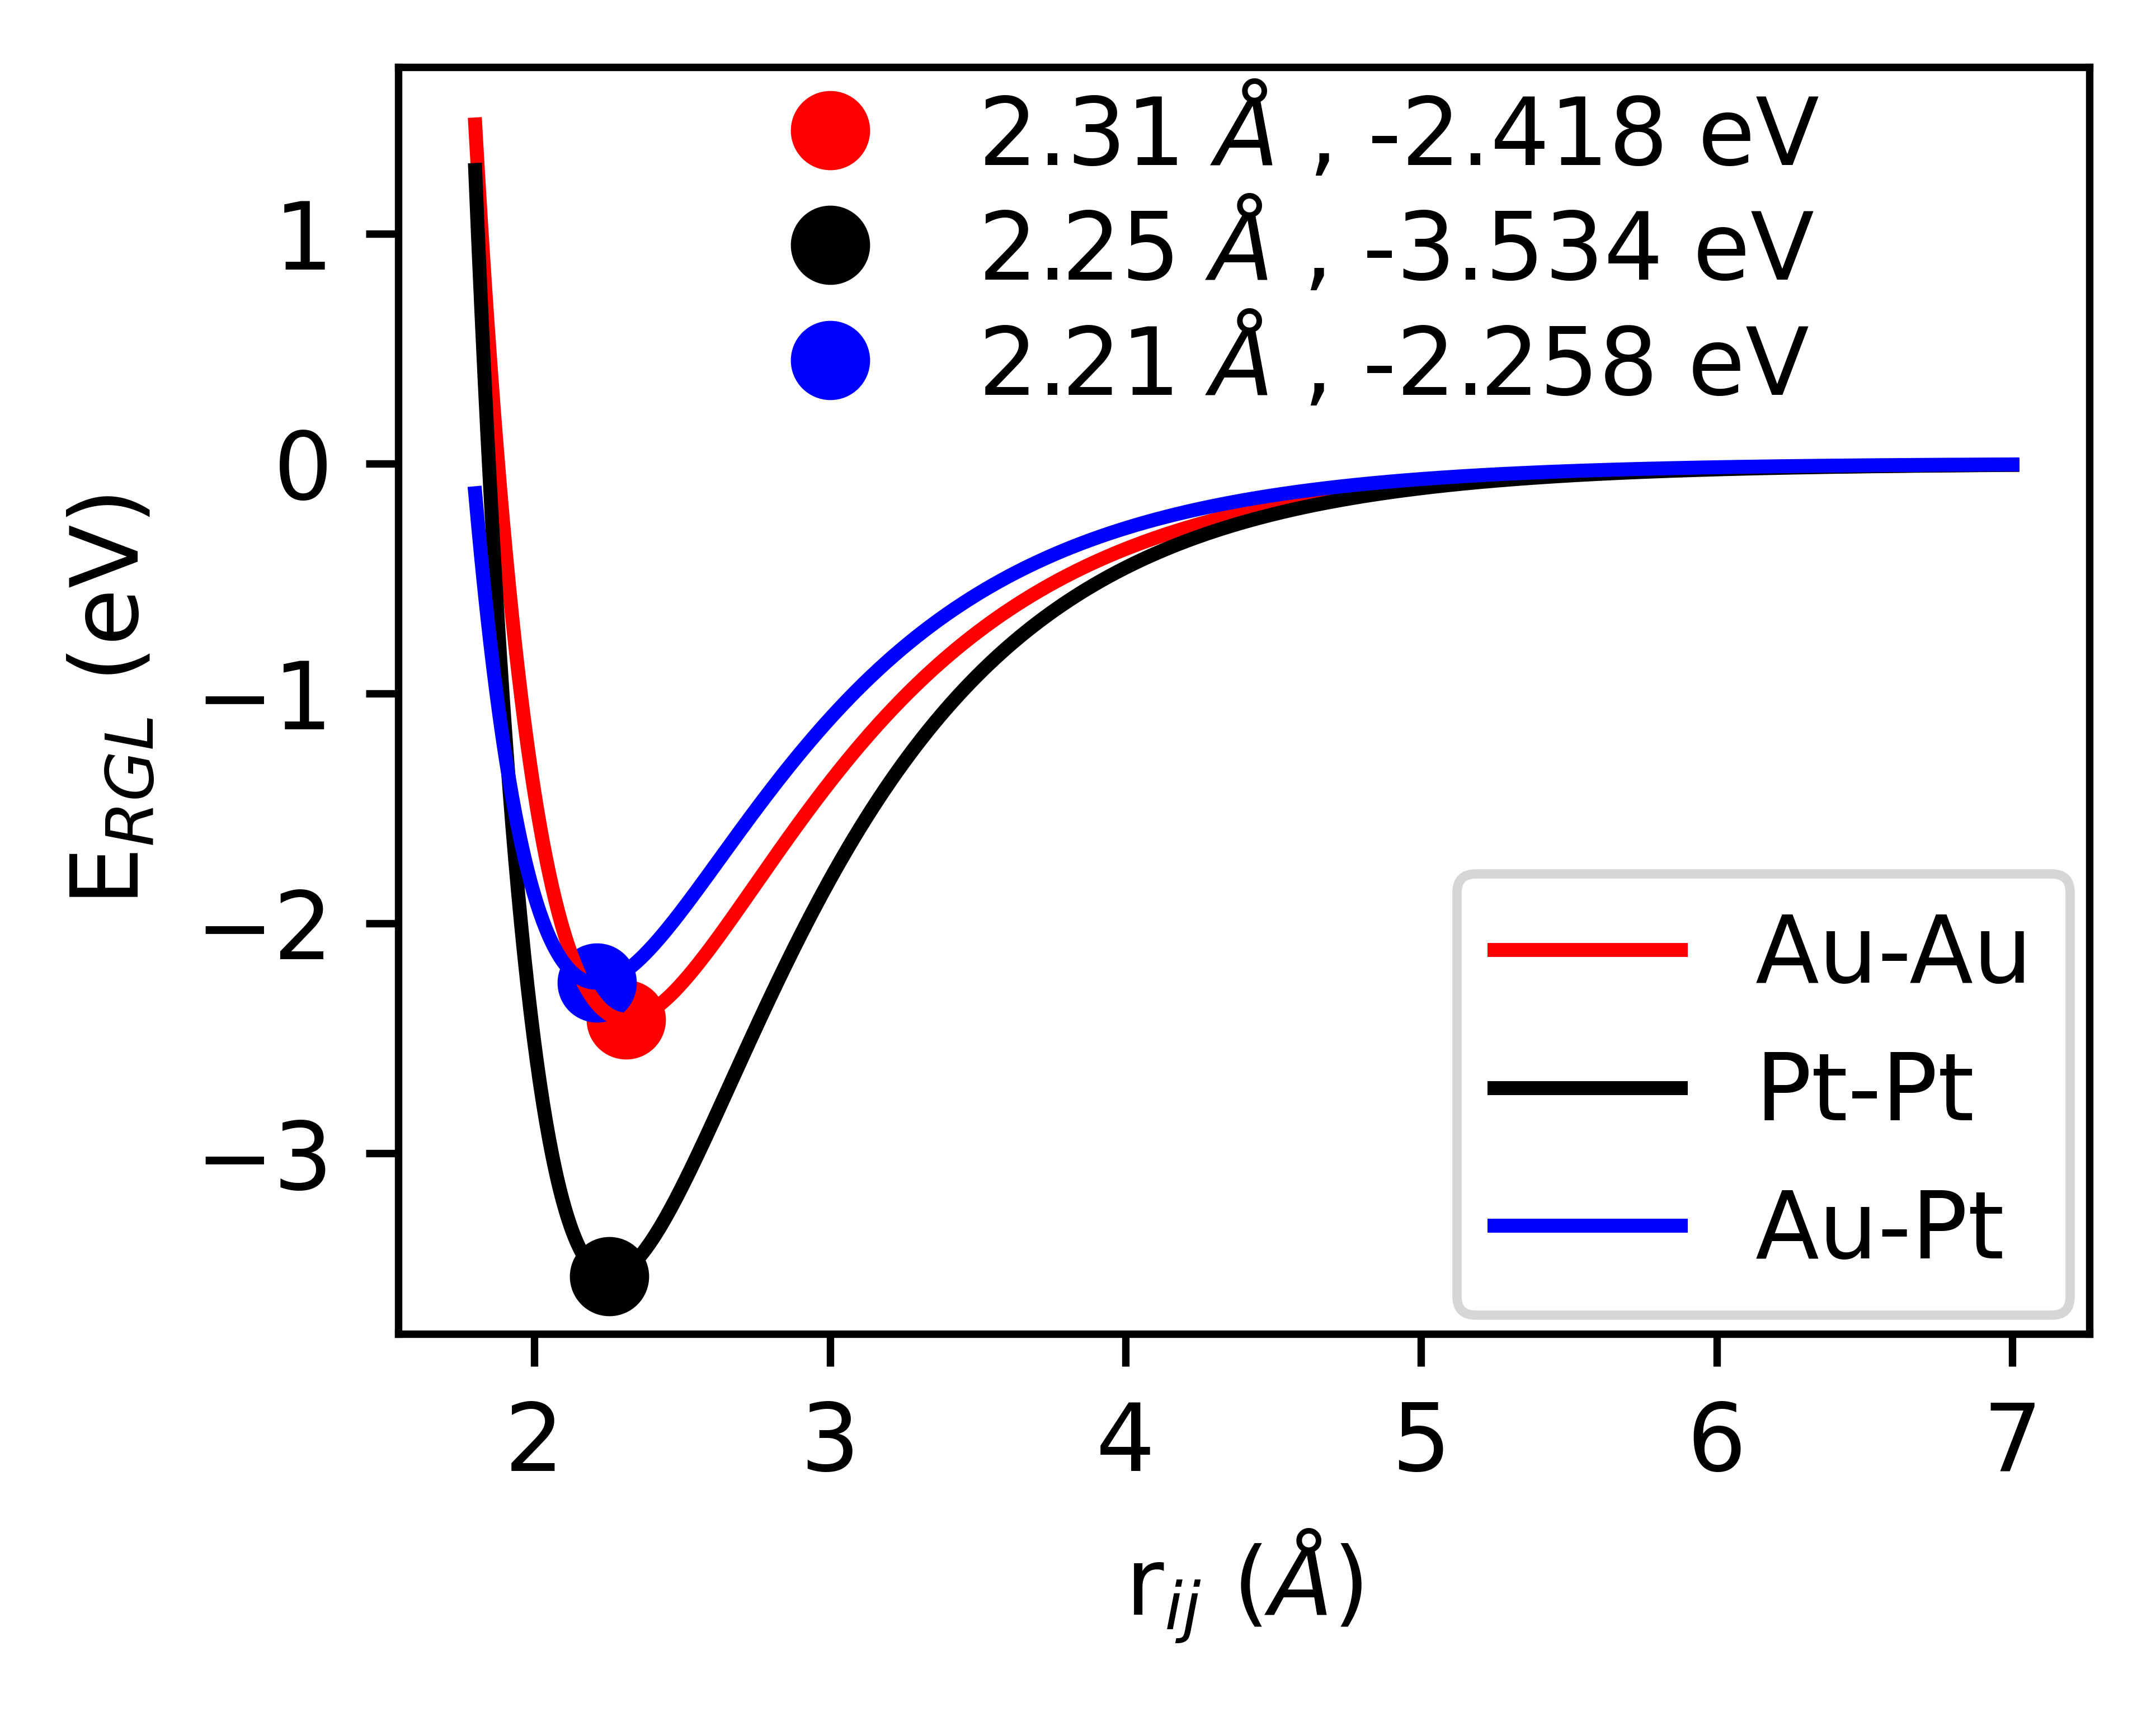
\includegraphics[width=\textwidth]{figures/Theory/Pots.png}
    \caption{Inter-atomic potentials.}
    \label{Fig:Gupta}
    \end{subfigure}
    \caption{Illustration of core components of a molecular dynamics (MD) simulation. (\textbf{a}) The thermostat, regulated by frequency of collisions (\textbf{i-iv}) and the temperature modulated by a Boltzmann distribution (\textbf{v}). (\textbf{b}) represents the potential energy landscape of the metallic species modelled in this project with the minima and their locations identified within the insert.}
    \label{Fig:Properties}
\end{figure}


\section{Density functional theory}
\label{sec:Theory_DFT}
An accurate representation of a nanoscale system must begin with the explicit electronic and ionic contributions to the many body Hamiltonian,
\begin{equation}
    H = \sum_{i} \frac{ P_{i}^{2} }{2m_{i}} + \sum_{I} \frac{ P_{I}^{2} }{2M_{I}} + \sum_{i>j} \frac{e^{2}}{ |\textbf{r}_{i} - \textbf{r}_{j}| } - \sum_{i,I} \frac{ Z_{I} e^{2} }{ | \textbf{r}_{i} - \textbf{R}_{I} |} + \sum_{I>J} \frac{ Z_{I}Z_{J}e^{2}}{ | \textbf{R}_{I} - \textbf{R}_{J} | }
    \label{eqn:MB_Ham}
\end{equation}
where lowercase scripts indicate electron quantities; capital letters indicate ion quantities; we work in natural units; and $Z_{I}$ is the proton number of the ion in question. This is fundamentally insoluble due to its many-body nature, namely the Coulomb interactions and complex structures of the nuclei that emerge from the combined effects of all the interactions. Our objective is to reconstitute this Hamiltonian in a fashion that treats electronic correlations with sufficient accuracy such that one may predict, with fidelity, the beautifully vast array of phenomena exhibited by matter, molecules, and clusters predicted by \ref{eqn:MB_Ham}\footnote{Note that phenomena such as magnetic fields, quantum electrodynamics, and relativstic effects are not included. Where appropriate, these will be addressed as we progress.}. Moreover, ion-ion interactions and ion-electron interactions further obfuscate what is already a daunting Hamiltonian. 

We directly address these issues by ignoring them. Or more precisely, we re-frame the question such that these issues never arise at all. In the following, we shall explore briefly the Kohn-Sham (KS) approach to the many electron problem \cite{KS}. This is to replace the complex, interacting system with an auxiliary system via an ansatz of our choosing ~- namely that the ground state density of the the original interacting system is equivalent to that of some chosen non-interacting system that may be considered soluble via numerical means. Whilst this is a powerful assertion, it alone is insufficient to make the problem more tractable, and requires subsequent approximations and generalisations before arriving at a system whose dynamics and properties are numerically tractable. When it is asserted that density functional theory (DFT) is ``inaccurate'', it is usually one of the myriad subsequent approximations that they are dissatisfied with as, in principle, density functional theory \textit{is} exact! In the subsequent subsections, we shall present and motivate a form of density functional theory which is practical, and serviceable for our needs.

\subsubsection{The ground state}
\label{sec:dft_gs}
Here, we will consider the KS ansatz for the ground state, the first port of call for any novitiate in the domain of DFT. More generally, it is the most ubiquitous component of the family of DFT calculations being performed. We begin by stating, without proof\footnote{One can prove these with basic variational arguments, and the exercise can be instructive as to the power and limitations of DFT.}, the so-called Hohenberg-Kohn theorems which provide a foundation upon which the theory rests.

\begin{theorem}
\label{thrm:HK1}
The external potential $v(\textbf{r})$ is determine, within an additive constant, by the electron density $\rho(\textbf{r})$. Since $\rho$ determines the number of electrons, it follows that $\rho$ determines ground state wave function $\Psi$ and all other electronic properties of the system. It is worth noting that the potential $v(\textbf{r})$ need not be restricted to Coulomb potentials.
\end{theorem}

\begin{corollary}
\label{cor:HK1}
Since the Hamiltonian is thus fully determined, except for some additive constant, it follows that the many-body wavefunctions for all states (ground and excited) are also determined. Therefore, all properties of the system are completely determined given only the ground state density $n_{0}(\textbf{r}$.
\end{corollary}

\begin{theorem}
\label{thrm:HK2}
A universal functional for the energy $E\left[ n \right]$ in terms of the density $n(\textbf{r})$ can be defined, valid for any external potential $V_{ext}(\textbf{r})$. For any particular $V_{ext}(\textbf{r})$, the exact ground state energy of the system is the global minimum value of this functional, and the density $n(\textbf{r})$ that minimises the functional is the exact ground state density $n_{0}(\textbf{r})$.
\end{theorem}

\begin{corollary}
\label{cor:HK2}
The functional $E\left[ n \right]$ alone is sufficient to determine the exact ground state energy and density. In general, excited states of the electrons must be determined by other means. Nevertheless, the work of Mermin shows that thermal equilibrium properties such as specific heat are determined directly by the free-energy functional of the density \cite{PhysRev.137.A1441}.
\end{corollary}

We note that nowhere in theorems \ref{thrm:HK1} and \ref{thrm:HK2} is there a requirement that the electrons be interacting, or that the many body contributions be explicitly considered. Therefore, we may invoke the KS ansatz which requires the two following assumptions:
\begin{enumerate}
    \item The exact ground state density can be represented by the ground state density of an auxiliary system of non-interacting particles. This is known as the ``\textit{non-interacting-V-representability};'' although there re no rigorous proofs for real systems of interest, it is generally considered to be valid. This leads to the relation between actual and auxiliary systems which is required.
    \item The auxiliary Hamiltonian is chosen to have the usual kinetic operator and an effective local potential $V_{eff}^{\sigma}(\textbf{r})$ acting on an electron of spin $\sigma$ at a position $\textbf{r}$. The local form is not essential\footnote{The original KS paper proposes an alternative approach with non-local orbital-dependent operators for exchange, to which effects of correlation are added \cite{KS}.} but is a useful simplification that is often used as the defining characteristic of the KS approach. We may assume that the external potential $\hat{V}_{ext}$ is spin independent;\footnote{For now, spin-orbit interactions are ignored.} nevertheless, except in cases that are spin symmetric, the auxiliary effective potential $V_{eff}^{\sigma}(\textbf{r})$ must depend on spin to give the correct density for each spin.
\end{enumerate}


\begin{figure}[ht!]
    \centering
    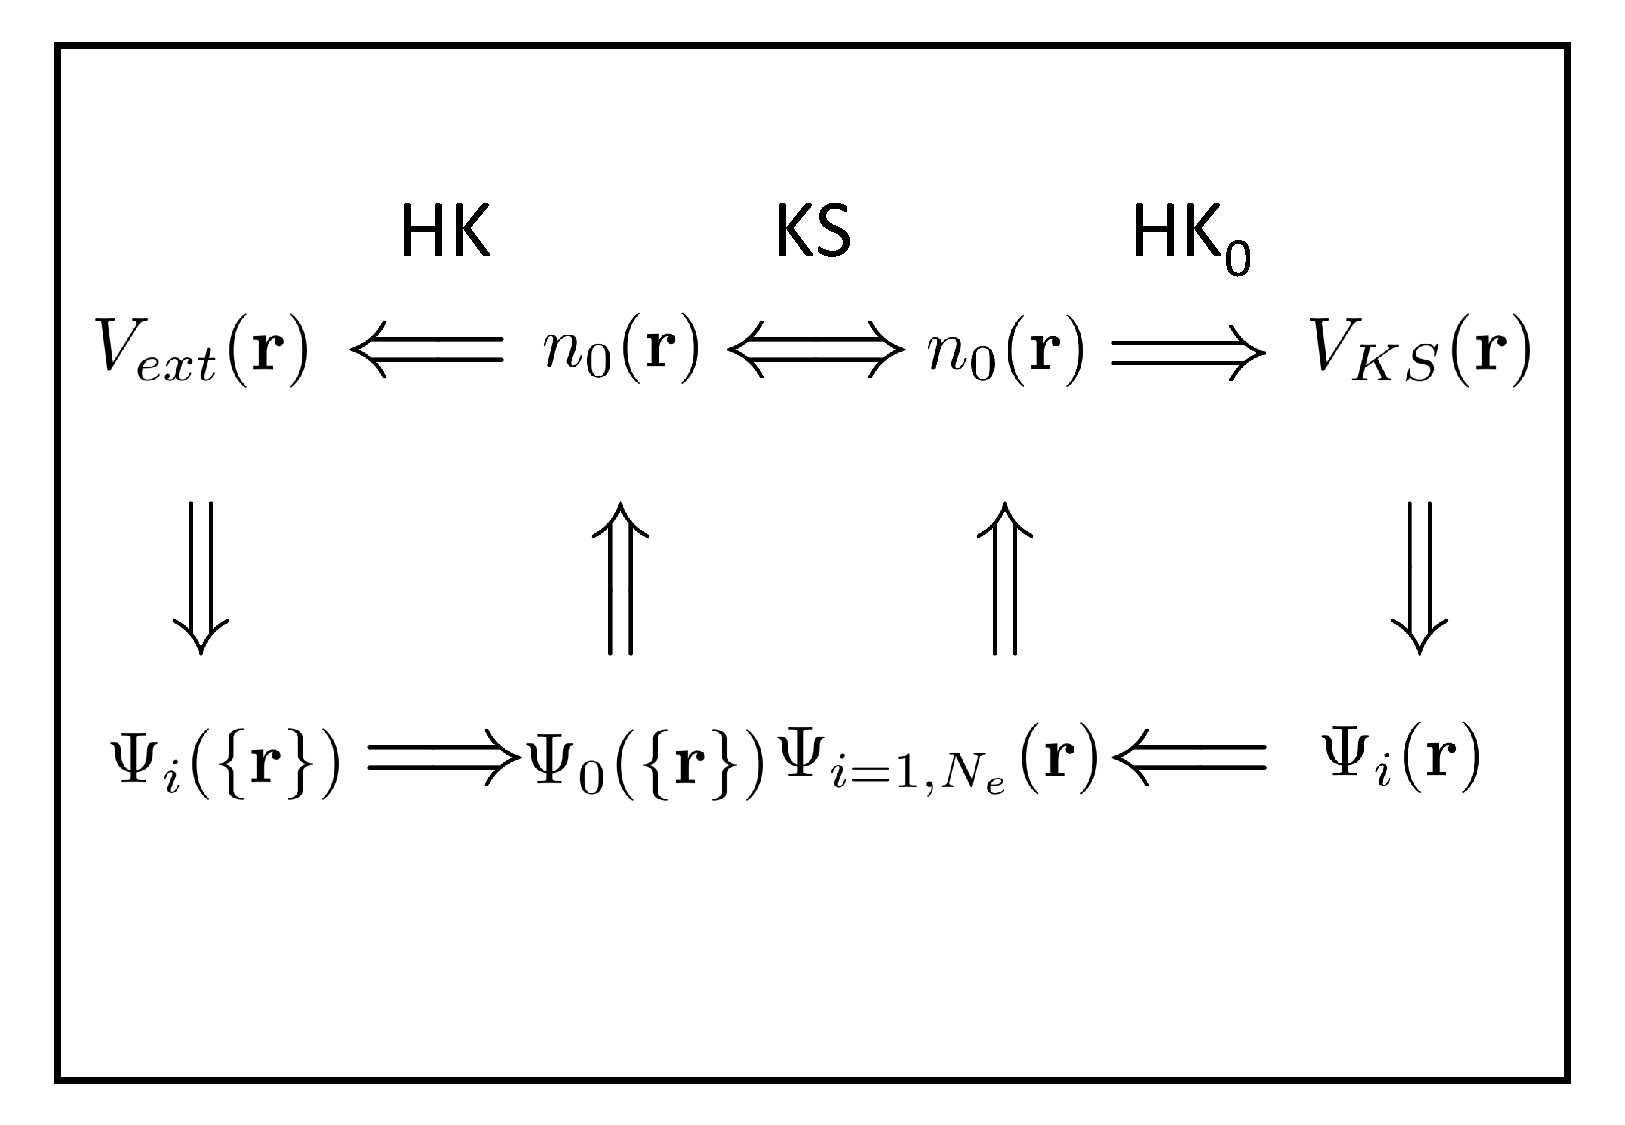
\includegraphics[width=0.95\linewidth]{figures/Theory/KS_ansatz.pdf}
    \caption{Illustration of the Kohn-Sham ansatz. HK$_{0}$ represents the non-interacting system and KS represents the connection between the interacting and non-interacting systems meaning that all points are connected. This diagram demonstrates how a solution to the non-interacting picture is also a solution to the interacting system.}
    \label{fig:my_label}
\end{figure}

With a full correspondence between the interacting and non-interacting auxiliary system, we may proceed to write down the simplified problem to be solved, namely the auxiliary Hamiltonian,

\begin{equation}
    \hat{H}^{\sigma}_{aux} = -\frac{1}{2}\nabla^{2} + V^{\sigma}(\textbf{r}).
    \label{eqn:dft_aux_ham}
\end{equation}

Despite the disarmingly simplistic appearance of the auxiliary Hamiltonian, equation \ref{eqn:dft_aux_ham}, we have nowhere specified thee form of $V^{\sigma}(\textbf{r})$, and the expressions must apply to all forms of $V^{\sigma}(\textbf{r})$ in some range if we are to successfully define functionals for a range of densities. For a system of $N= N^{\uparrow}+N^{\downarrow}$ independent electrons obeying thsi Hamiltonian, the ground state has one electron in each of the $N^{\sigma}$ orbitals $\psi_{i}^{\sigma}(\textbf{r})$ with the lowest eigenvalues 

\subsubsection{Functionals}
\label{sec:dft_funk}

We now come to address the electron~-~electron term interaction. Skipping over decades of development\footnote{An instructive discussion of the progression of wavefunction methods, such as Hartree~-~Fock, are provided in Ashcroft and Mermin \cite{Ashcroft76}.}, one solution to this many body problem is to split this potential term into two separate terms: the Hartree potential and the exchange-correlation potential,

\begin{equation}
    V_{H}[n](\textbf{r}) = \int \frac{ n(\textbf{r'}) }{ |\textbf{r} - \textbf{r'} | } d\textbf{r'} \text{ and } V_{XC}[n](\textbf{r}) = \frac{\delta E_{XC} }{\delta n(\textbf{r})}.
    \label{eqn:VHVXC}
\end{equation}

Unfortunately, $V_{H}[n](\textbf{r})$ is a pathological function and cannot be analytically solved, and $V_{XC}[n](\textbf{r})$ is a fundamentally unknowable functional derivative of the exchange-correlation energy, $E_{xc}$, with respect to the density. Typically, one will use either the local density approximation (LDA) \cite{KS} or generalised gradient approach (GGA) \cite{Purdue_Yue_GGA,GGA_Simple}, which are explicit functionals of the density and its gradient. However; there are alternatives emerging, such as the use of orbital dependent functionals which are only implicit functionals of the density. In the proceeding work, we shall be working within both the LDA and GGA formalism of density functional theory (DFT) depending on the system under consideration. It is worth noting that the benefit of introducing the potentials in Equation \ref{eqn:VHVXC} allows us to rewrite the many-body problem of Equation \ref{eqn:MB_Ham} as non-interacting, non-linear problem. This is computationally cheaper to solve, and indeed allows the appropriate communities to handle such systems at a larger scale.

The true beauty of Kohn Sham (KS) DFT is that it is exact. However; this comes with the caveat implied above, the functionals which formulate DFT are unknowable and pathological, and so necessary approximations dilute the exactness of the theory to \textit{sufficiently representative}.

As previously discussed, the method of combining all of the fundamentally unknowable potentials into the exchange-correlation term necessitates its approximation. As such, there is no `physical' lower bound for what the total energy of the system ought to be minimised to. That is to say that the quality of the calculation will only be as accurate as the selected potentials. Moreover, in Hartree-Fock theory, the true ground state of the system provides a lower bound for minimisation via the variational principle. However, in KS DFT, the arbitrary choice of $V_{xc}$ violates the physical onditions meaning that the minimisation of the eigenvalue problem in the KS formalism is not necessarily physically representative of a real system. This provides a scientific imperative to ensure that both experimental and computational communities communicate sufficiently to ensure that calculations performed via KS DFT methods are as faithful to experimental data as can be achieved given the pathologies of the functionals contributing to contemporary DFT.
We now address the nature of the external potential, as the descriptions thereof form a crucial component of modern DFT calculations. For larger ions, those which are more accurately modelled under the BOA, there exist many electrons which are tightly bound to the atomic nucleus. In principle, one should explicitly consider the contributions of all so-called core electrons to the calculated density. Indeed, these calculations are regularly performed and are known as `all-electron' calculations. However; it should be evident that including hundreds or even thousands of additional electrons whose participation in chemical interactions are negligible will largely serve to retard any computation with minimal gain in accuracy. A convenient solution to this dilemma is to incorporate the electrostatic properties of these core electrons into the external potential created by the ions. This is the heart of the use of pseudopotentials in DFT methods. Because core electrons are tightly bound to the nucleus by strong Coulomb potentials, their wavefunctions are highly localised around their parent nucleus, and their energies are both large and negative. Here we introduce the frozen-core approximation, in that while the energies of the core electrons may vary slightly in alternative environments, such as in a suspension or crystal, the shape of their wavefunctions are, to a sufficient degree of accuracy, assumed to be identical to that of an isolated atom. 

Herein emerges an issue with the use of pseudopotentials, to respect the quantum mechanical nature of the system, all electron wavefunctions must be mutually orthogonal. This results in the nodal structure of the valence electron wavefunctions in that it will oscillate rapidly in the core region. This is an issue as a greater number of basis functions are required to accurately reproduce this wavefunction shape within the core which would only serve to further retard a calculation. One method of circumventing this problem is to introduce a smoothing to the valence orbitals within the core region. This is an inherently fictitious caricature of how the valence electrons' wavefunctions will appear. However; under the proviso that their shape outside of the core region is identical to that of the wavefunction prior to modification. This is motivated by the same rationale which underpins the frozen-core approximation - in that all of the 'interesting' physics and chemistry occurs beyond the tightly bound states. 


\subsubsection{Pseudopotentials}
\label{sec:Ps}
In a fashion consistent with the ideas of DFT, a standard method of handling the strong Coulomb potential of the atomic nuclei and the tightly bound core electrons is to simply ignore the actual challenge. Or more accurately, one replaces the issue of considering nuclei and core electrons with a more tractable, effective ionic potential. Moreover, the variability in how one may introduce pseudopotentials grants an additional freedom to choose forms that better suit the nature of a given calculation being performed, and subsequently the interpretation of the resultant electronic structure.

In principle, one should explicitly consider the contributions of all so-called core electrons to the calculated density. Indeed, these calculations are performed, and are known as `all-electron' calculations. However; it should be evident that including hundreds or even thousands of additional electrons whose participation in chemical interactions are negligible will largely serve to retard any computation with minimal gain in accuracy. A convenient solution to this dilemma is to incorporate the electrostatic properties of these core electrons into the external potential created by the ions. This is the heart of the use of pseudopotentials in DFT methods. Because core electrons are tightly bound to the nucleus by strong Coulomb potentials, their wavefunctions are highly localised around their parent nucleus, and their energies are both large and negative. Here we introduce the frozen-core approximation, in that while the energies of the core electrons may vary slightly in alternative environments, such as in a  suspension or crystal, the shape of their wavefunctions are, to a sufficient degree of accuracy, assumed to be identical to that of an isolated atom. 

Herein emerges an issue with the use of pseudopotentials, to respect the quantum mechanical nature of the system, all electron wavefunctions must be mutually orthogonal. This results in the nodal structure of the valence electron wavefunctions in that it will oscillate rapidly in the core region. This is an issue as a greater number of basis functions are required to accurately reproduce this wavefunction shape within the core which would only serve to further retard a calculation. One method of circumventing this problem is to introduce a smoothing to the valence orbitals within the core region. This is an inherently fictitious caricature of how the valence electrons' wavefunctions will appear. However; under the proviso that their shape outside of the core region is identical to that of the wavefunction prior to modification. This is motivated by the same rationale which underpins the frozen-core approximation - in that all of the 'interesting' physics and chemistry occurs beyond the tightly bound states. In the following work, 


\subsubsection{Auxiliary and numerical considerations}
\label{sec:dft_nums}

DFT is a well established method of obtaining ground state properties of quantum mechanical systems and its description via the KS framework has emerged as the primary method for performing \textit{ab initio} calculations \cite{K_Burke_Perspectives,Becke_Perspective}. Without loss of generality, one must provide an initial prior on what the electron density of a system may be. This can be done in a manner of different ways, each with their own merits, however the common theme is that a single scheme is chosen as to how electrons are to be modelled. For example, some DFT packages such as Gaussian will describe the wavefunction of each electron as a Gaussian wavepacket. The initial electron density, $n(\textbf{r})$ at position $\textbf{r}$, of this system may then be represented as the normalised superposition of these electron wavefunctions, ${\varphi_{i}(\textbf{r})}$ where the index i runs over all of the electron wavefunctions. With a trial density, equation \ref{eqn:dens}, one proceeds to construct the one-particle KS equations.

\begin{equation}
    h_{KS}\varphi_{i}(\textbf{r}) = \varepsilon_{i}\varphi_{i}(\textbf{r}) \text{ such that } h_{KS}[n] = -\frac{1}{2}\nabla^{2} + V_{ext}(\textbf{r}) + V_{H}[n](\textbf{r}) + V_{XC}[n](\textbf{r}) 
    \label{eqn:hKS}
\end{equation}

Note that KS operator, $h_{KS}$, is explicitly a function of the electron density,
\begin{equation}
    n_{0}(\textbf{r}) = \sum_{i}^{N} |\varphi_{i}(\textbf{r})|^{2}.
    \label{eqn:dens}
\end{equation}. 
This is the precise reason that an initial density is required at the commencement of any DFT calculation. With the KS operator and trial density from trial wavefunctions, one may then iterate the self consistent field (SCF) calculations to an arbitrary convergence. The convergence criterion is defined by
\begin{equation}
    \frac{1}{N}  \int_{\mathbb{R}^{3}} d^{3}x \left| n^{(out)}(x) - n^{(inp)}(x)  \right|   \leq x
    \label{eqn:conv}
\end{equation}
where $x$ is the tolerance used for the specific calculation. This is typically set such that the maximal variation for any given electron's density during an SCF cycle is $x\leq10^{-6}$. To be precise, we shall describe the notion of `convergence' to be the condition met when the input density is sufficiently alike to the output density so as to consider an accurate representation of the 'true' density to have been found. Granted, this does not necessarily preclude landing in local minima. However, schemes exist within the framework of DFT to ensure that the phase space is sufficiently sampled in consideration of this problem.

There still remains the issue that each of these SCF cycles requires the solving of large matrices. A problem which, in principle, may scale as $\mathcal{O}(N^{3})$ for dense matrices with no exploitable symmetries. This is devastating when systems of interest may easily contain thousands of electrons. 

At this point, we acknowledge the utility of the real-space feature of the code we are utilising for this work, Octopus \cite{Octopus2003,Octopus_2006}. In real space, the problem of solving the Hamiltonian is alleviated as the matrix becomes sparse meaning that more efficient algorithms may be implemented. We primarily have used conjugate gradient based approaches as we have found this to lead to the smoothest and most reliable SCF processes.

A further tool often used to ensure convergence of the SCF process is to introduce a mixing parameter which makes a subsequent density a superposition of the previously returned densities. In general,

\begin{equation}
    n^{(i+1)} = \mathbf{F}\left[n^{(i)}, n^{(i-1)}, ..., n^{(init)} \right]
\end{equation}
however the simplest solution is to simply have a linear combination of the previous density. For our calculations, we have utilised the more sophisticated Broyden scheme \cite{Oct_2020}.

Having reached convergence, it is worth being aware of what one has actually calculated. With a ground state density, one has access to the full density of states for their structure, magnetic properties if spins were taken into consideration and the KS eigenvalues. Typically, the eigenvalues of a Hamiltonian may be considered to be its energy spectrum. This, however, is not the case in KS DFT, as the one-electron eigenspectrum indeed has no physical meaning. What is meaningful is a given energy difference. Indeed, this means that the ionisation potential may be stated as the energy of the highest occupied orbital in the system in accordance with Koopman's theorem. However, this is not necessarily the case for deeper states.


\subsection{Jellium Model}
\label{sec:JML_Thr}
To briefly motivate the origins of using the Homogeneous Electron Gas (HEG), hereafter referred to as Jellium, within the context of metallic nanoparticles - a series of mass spectra experiments on alkali metals conducted by Knight \textit{et al.} \cite{Knight_Cluster} revealed an enhanced stability of clusters with specific nuclearities. Increased stability was indicated by sharp peaks in the mass spectrum data relative to neighbouring data points, and the corresponding mass values were appropriately named magic numbers.

Initially, the Jellium model was used to account for the stability of these structures, it has since been used to describe the electronic structure of the atom and has been identified as a model whose applicability traverses a range of size scales from the inside of a nucleus to clusters many nanometers in size.

In the spherical Jellium model, a cluster is modelled by a uniform, positively charged sphere filled with an electron gas. Solving this system requires the assumption that the electron moves under the influence of an attractive mean field potential due to the ions whose positions are not important within the Jellium model. This assumption turns out to be surprisingly accurate in the case of the outer valence electron being weakly bound to its progenitor ion. This is true in the case of the outer electron having a strong $s$-type character, such as for the alkali and noble metals.

At its core, the Jellium model is inherently quantum mechanical whereby electron energy levels are quantised due to the boundary conditions imposed by the potential. In principle, the Jellium potential may be empirical, although it is more common for \textit{ab initio} methods to be implemented as a means of evaluating the potential. This may by done by solving Hartree-Fock molecular orbitals - however it is far more common to use the cheaper alternative of DFT.

A homogeneous system may be completely defined with respect to the density of its charges, $n_j$, which is determined by the parameter $r_{s}$, the radius of a sphere containing a single electron. Effectively, this radius is the Wigner-Seitz cell radius - defined as the radius of a sphere whose volume is equal to the volume of a single atom. Given the self-imposed restraint to model only noble and alkali metals with a single valence electron with an $s$-type character, this cell radius is readily interpreted as stated above. Given this radius and sphericity condition, the density is given as,

\begin{equation}
    n = \left( \frac{4\pi r^{3}_{s}}{3} \right)^{-1}.
\end{equation}

By replacing the ion term in eqn. \ref{eqn:MB_Ham} with a uniform positively charged density, the Jellium Hamiltonian may be rewritten as,

\begin{equation}
    H = \sum_{i} \frac{ P_{i}^{2} }{2m_{i}} + \frac{1}{2} \left[ \sum_{i \neq j} \frac{e^{2}}{ |\textbf{r}_{i} - \textbf{r}_{j}| } - \int d^{3}rd^{3}r^{\prime} \frac{(ne)^2}{|\textbf{r} - \textbf{r}^{\prime}|} \right],
    \label{eqn:jlm}
\end{equation}

where we note that the final term is the average background density introduced to cancel out the divergence due to the Coulomb interaction between the electrons. We may proceed to write out the total energy in the Jellium model in a similar fashion to Equation \ref{eqn:hKS} such that 

\begin{equation}
    E = \langle H \rangle = \langle T \rangle + \langle V_{int} \rangle - \frac{1}{2} \int d^{3}rd^{3}r^{\prime} \frac{(ne)^2}{|\textbf{r} - \textbf{r}^{\prime}|}
    \label{eqn:jlm_E}
\end{equation}

where $\langle T \rangle$ is the kinetic energy of the electrons within the model, and the final two terms are the difference in the potential energy of these electrons and the self-interaction of a uniform charge density. 

With a well defined energy and electron density, proceeding to compute time dependent properties within the Jelllium is no different than in the prescription detailed earlier. 

\subsection{Time dependant density functional theory}
\label{sec:RTTDDFT}
\subsubsection{Real time propagation}
\label{sec:TDDFT_Thr}
To obtain optical and electronic properties at the quantum mechanical theory level, we have used the code of Octopus 11.1 \cite{Octopus2003,Octopus_2006,Oct_2015,Oct_paralel,Oct_2020} - a real-space DFT suite of codes designed for determining the spectroscopic details of finite systems via both linear response and real time propagation schemes. All of our calculations have been performed within the local density approximation (LDA) \cite{KS} using norm-conserving pseudopotentials of the Hammann \cite{Hamann} and Troullier-Martins \cite{Troullier} types \cite{FHI} which have permitted us to perform spin-polarised calculations to better capture the exotic phenomena presented by the NAs. We have discretised the real space grid into cubic units of $(0.1$\AA$)^{3}$ which approximately corresponds to a plane-wave cutoff of 276.4~Ry. Our mesh is constructed by placing a sphere of radius $5$ \AA \ around each atom, constructed from a collection of grid units. To achieve better convergence of the ground state density, we smooth the Fermi-Dirac distribution with a cold smearing function \cite{Smearing} set to 1 meV.

A standard method of obtaining the absorption spectrum is via the quasi-static dipole approximation in that an instantaneous perturbation may be applied to the ground state density of the system at a time $t_{0}$ which takes the form, 
\begin{equation}
    \textbf{E}(\textbf{r},t) = K_{0}\delta(t)\textbf{u} = \frac{1}{\pi} \int_{0}^{\infty}d\omega~K_{0}\cos{\omega t} \textbf{u},
\end{equation}
essentially white light polarised along the vector $\textbf{u}$ with incident intensity $K_{0}$. This perturbation results in an instantaneous transfer of momentum to the system which is then permitted to evolve under its own dynamics \cite{Yabana1996}.


In principle, the optical absorption spectrum tensor may be directly calculated from the Fourier transform of the induced dipole moment, $\mathbf{d}(t)=\int  \mathbf{r}\delta n(\mathbf{r},t) d\mathbf{r}$, with respect to time,
\begin{equation}
    \hat{\sigma}_{\textbf{u}}(\omega) = - \frac{\omega}{\pi K_{0}}  \Im \int_{0}^{\infty} dt e^{ (i\omega -\eta)t } \left(\textbf{u}\otimes \mathbf{d}(t)\right)
    \label{eqn:DFTSigma},
\end{equation}
where $\eta$ is some positive infinitesimal. We note that to obtain the optical spectrum, we need only know about the induced dipole density, and thus the induced electron density, $\delta n(\mathbf{r},t)$. The latter is the difference between the density at time $t$ and at the initial time (usually that of the ground state) such that
\begin{equation}
    \delta n(\textbf{r}, t) = n(\textbf{r}, t) - n(\textbf{r},0).
    \label{eqn:dense}
\end{equation}

To compute the full polarisability tensor and, by extension the absorption spectrum, the dipole response must be calculated with respect to three spatially orthonormal vectors $\textbf{u}$. Whenever the perturbation is sufficiently small, the theory is equivalent to the standard linear response approach, based for example, on the Casida's equations \cite{Casida} (see for instance, the user manual of Octopus for a comparison between the methods).  

Given that a Fourier transform is employed in the computation of equation \ref{eqn:DFTSigma}, one observes that the length of simulation essentially sets the resolution in frequency space, and so longer propagations will yield in more highly resolved spectra which provides a finer resolution for computed spectra. While the size of the time increment may serve only to unlock higher, and largely unnecessary frequencies, it is worth keeping in mind that large time steps may result in numerical instabilities during propagation.  

Moreover, one may note in equation \ref{eqn:DFTSigma} that the tensor for which we only consider the imaginary component of is indeed the dynamical polarisability tensor. This observation may then lead one to conclude that to have an accurate polarisability tensor, one must consider the dipole response with respect to three spatially orthonormal vectors. This is indeed the case, however one may utilise any symmetries present in their system to reduce the need for additional calculations.

This is indeed true for small, instantaneous perturbations. However; in the case of a simulated laser field, incident fields may be large and there is no guarantee that illumination will be instantaneous. Hence, the probability of ionisation or single electron excitations becomes increasingly non-zero. Such induced potentials may be considered to typically take the form,

\begin{equation}
    V(\textbf{r},t) = E_{0}f(t)\text{sin}(\omega t)\Hat{\textbf{P}}\cdot \textbf{r}
    \label{eqn:pulse}
\end{equation}
in which the time dependent function, $f(t)$, is the envelope function for the pulse polarised along the vector $\Hat{\textbf{P}}$ with frequency $\omega$ and intensity $E_{0}$. In this instance of an arbitrarily strong and sustained laser pulse, the perturbative method would be inaccurate and so the method commonly used is to analyse the high harmonic generation (HHG) spectrum of the system as this may include multiple photon excitations with an electron relaxing by emitting a single photon being an integer multiple in energy of the incident radiation. By neglecting coherent processes, one may approximate the emission spectrum from the acceleration of the dipole moment, $\Hat{\textbf{R}}$, as

\begin{equation}
    \sigma_{emission}(\omega) = \left| \int dt e^{-i\omega t}\frac{d^{2}}{dt^{2}} \langle \Hat{\textbf{R}} \rangle \right|^{2}
    \label{eqn:HHG}
\end{equation}
which has the advantage of being simple to calculate from a TDDFT calculation \cite{Oct_2015}.

Having converged a system to a sufficiently accurate ground state, the next task is to calculate optical properties. This may be done in one of several ways. We shall briefly discuss the Casida formalism as this is pertinent to single electron excitations. However, the factorial scaling built into solving the Casida equations renders it sub-optimal for the scale and range of systems we study. Alternatively, we shall be exploring and motivating real time time dependent DFT (RT-TDDFT) techniques which require propagating the Hamiltonian in time. It is a somewhat trivial thing to re-tool the KS equations into a time-dependent form. One acknowledges that as electrons undergo their own dynamics, the potentials they create will too change dynamically. Moreover, one may also introduce the notion of external potentials in the form of electromagnetic coupling with electrons. We write the time dependent KS (TDKS) equations below,

\begin{equation}
    i \frac{\partial}{\partial t} \varphi_{i}(\textbf{r},t) = h_{KS}[n(\textbf{r},t)](t)\varphi_{i}(\textbf{r},t),
    \label{eqn:TDKS}
\end{equation}
in which all of the terms from equation \ref{eqn:hKS} are given explicit time dependence. In principle, the exchange-correlation term should have memory in that it explicitly depends on all densities at all times in the past. This is evidently impracticable from a computational perspective. Moreover, there does not exist a well defined functional explicitly for TDDFT which sufficiently incorporates the time dependent nature of the evolution of the electron density. Therefore, it is standard practice to employ the adiabatic approximation in which one writes
\begin{equation}
    V_{XC}[n](\textbf{r},t) = V_{XC}^{gs}[\rho]|_{\rho = n(\textbf{r},t)},
    \label{eqn:adiabaticVxc}
\end{equation}
such that the form of the exchange-correlation potential remains unchanged and is simply fed a new density at each time step to recalculate.

Here, one is forced to appreciate the magnitude of the task in computing the unitary time evolution operator,
\begin{equation}
    \varphi(\textbf{r}, t+\Delta t) = \Hat{U}(t+\Delta t, t)\varphi(\textbf{r},t)
    \label{eqn:UTO}
\end{equation}
where we must use the full expansion of the time evolution operator as the Hamiltonian is itself explicitly time dependent. Even in the absence of external fields, due to the presence of the Hartree potential,

\begin{equation}
    \Hat{U}(t+\Delta t, t) = \sum_{n}^{\infty} \frac{(-i)^{n}}{n!} \int_{t}^{t+\Delta t} dt_{1} ... \int_{t}^{t+\Delta t} dt_{n} \mathcal{T}\left[ h_{KS}(t_{1}) ... h_{KS}(t_{n}) \right],
    \label{eqn:UTE}
\end{equation}

where $\mathcal{T}$ defines the time ordering operator. There exist many methods of approximation for this infinite expansion, most of which consist of polynomial expansions. In truth, the method used is secondary to the consideration of the task involved in expanding this operator for an already cumbersome Hamiltonian.

\subsubsection{Nuclear motion}
\label{sec:nuclear_motion}

Having otherwise discussed time-dependent dynamics, we have neglected the elephant in the room ~- that of how the ions may move in the presence of an external potential, or changes in the electronic potentials. To now, we have implicitly assumed that nuclei may be modelled to be fixed at their equilibrium positions, treating them as classical point charges. However, nuclei are still fundamentally quantum mechanical particles, and the full wavefunction should reflect this reality. Not only does this mean that nuclear motion must be considered with respect to other nuclei, but so too must the coupling between nuclei and electrons be considered. Therefore, it is essential that any model which incorporates nuclear degrees of freedom into the model must use well physically motivated, yet powerful approximations to handle the coupled dynamics. 

This section will begin with a reassessment of the electronic-nuclear problem, and continue by motivating how one may decouple electronic and nuclear degrees of freedom ~- presenting standard arguments. We shall then progress to presenting and motivating several common methods of propagating nuclear motion in a real time scheme

We begin by take introducing the Born-Oppenheimer approximation (BOA) to decouple the electronic and ionic degrees of freedom as the mass ratio between the two is vanishingly small. We may begin by rewriting the starting Hamiltonian, \ref{eqn:MB_Ham}, as

\begin{equation}
    \hat{H} = \hat{T}_{N} + \hat{T}_{e} + \hat{U},
    \label{eqn:boa_init}
\end{equation}
where $\hat{U}$ contains all of the potential interaction terms involving the set of all-electron coordinates $\{ \mathbf{r} \}$, and the set of nuclear coordinates $\{  \mathbf{R} \}$. Due to the typically larger mass of the nuclei, the nuclear kinetic term $\hat{T}_{N}$ is typically small, we may treat it as a perturbation on the Hamiltonian \ref{eqn:boa_init} for nuclei fixed in their instantaneous positions. We now write out the eigenspectrum of the Hamiltonian for the electrons which depend on the nuclear positions $\{ \mathbf{R} \}$ as parameters, $E_{i}( \{ \mathbf{R} \} ) $ and $\psi_{i}(\{ \mathbf{r} \} : \{ \mathbf{R} \})$ with the indices $i$ denoting the complete set of states for each $\{ \mathbf{R} \}$. This full solution may be rewritten as,

\begin{equation}
    \hat{H} \psi_{s}(\{ \mathbf{r}, \mathbf{R} \}) = E_{s}\psi_{s}(\{ \mathbf{r}, \mathbf{R} \}),
    \label{eqn:boa_coupled_init}
\end{equation}
where $s=1,2,3...,$ describes the states of the coupled system, can be written in terms of $\psi( \{ \mathbf{r} \}: \{ \mathbf{R} \}$,

\begin{equation}
    \psi_{s}(\{ \mathbf{r}, \mathbf{R} \}) = \sum_{i}\chi_{si}(\{ \textbf{R} \} ) \psi_{i}(\{ \mathbf{r}: \mathbf{R} \}),
    \label{eqn:boa_coupled_final}
\end{equation}

since $\psi_{i}(\{ \textbf{r} \} : \{ \textbf{R} \} )$ defines a complete set of states for the electrons at each $\{ \textbf{R} \}$. Furthermore these states, $\psi_{s}(\{ \textbf{r}, \textbf{R} \})$, are specified by $\chi_{si}(\{ \textbf{R} \} )$, functions of the nuclear coordinates and are the coefficients of the electronic states. To resolve these functions, we may begin by inserting the expression for $\psi_{s}$ (\ref{eqn:boa_coupled_final}) into the wavefunction equation (\ref{eqn:boa_coupled_init}), multiply from the left by $\psi_{i}( \{ \textbf{r}, \textbf{R} \})$, and integrate over the electron coordinates $\{ \textbf{r} \}$ to arrive at the following expression,

\begin{equation}
    [ T_{N} + E_{i}( \{ \textbf{R} \}) - E_{s} ] \chi_{si}(\{ \textbf{R} \}) = - \sum_{i'}C_{ii'}\chi_{si'}(\{ \textbf{R} \}),
    \label{eqn:boa_cont}
\end{equation}

where $T_{N} = - \frac{1}{2} \left( \Sigma_{J} \nabla_{J}^{2} / M_{J} \right)$ and the matrix elements are given by $C_{ii'}=A_{ii'} + B_{ii'}$ with

\begin{equation}
    A_{ii'}(\{ \textbf{R} \} ) = \sum_{J} \frac{1}{M_{J}} \bra{\psi_{i}(\{ \textbf{r} \} : \{ \textbf{R} \})} \nabla_{J} \ket{ \psi_{i'}(\{ \textbf{r} \} : \{ \textbf{R} \}) } \nabla_{J},
    \label{eqn:boa_A}
\end{equation}

\begin{equation}
    B_{ii'}(\{ \textbf{R} \} ) = \sum_{J} \frac{1}{2M_{J}} \bra{\psi_{i}(\{ \textbf{r} \} : \{ \textbf{R} \})} \nabla_{J}^{2} \ket{ \psi_{i'}(\{ \textbf{r} \} : \{ \textbf{R} \}) }.
    \label{eqn:boa_B}
\end{equation}

Where $ \bra{\psi_{i}(\{ \textbf{r} \} : \{ \textbf{R} \})} \mathcal{O} \ket{ \psi_{i'}(\{ \textbf{r} \} : \{ \textbf{R} \}) }$ is an integration over only the electronic coordinates $\{ \textbf{r} \}$ for any operator $\mathcal{O}$.

This is where we get to the meat and potatoes of the BOA; all off-diagonal contributions to $C_{ii'}$ are neglected. Essentially, this assumes that the electrons remain in a given state $m$ during ionic motion. Despite the fact that the electronic wavefunctions $\psi_{i}(\{ \textbf{r} \} : \{ \textbf{R} \} )$ and the energy of state $m$ change, the electrons do not change state and no energy is transferred between the degrees of freedom described by the equation for the nuclear variables $\{ \textbf{R} \}$ and excitations of the electrons, which occurs if and only if there is a change of state $ i \rightarrow i'$. As for the idagonal terms, we first note that $A_{ii} = 0 \forall i$ from the requirement that $\bra{\psi}\ket{\psi} = 1$. Furthermore, $B_{ii}(\{\textbf{R}\})$ may be grouped with $E_{i}(\{\textbf{R}\})$ to determine a modified potential function for the nuclei $U_{i}(\{ \textbf{R}\}) = E_{i}(\{ \textbf{R}\}) + B_{ii}(\{ \textbf{R}\})$. Therefore, within the BOA, the nuclear motion is described by a purely nuclear equation for each electronic state $i$.

\begin{equation}
    \left[ 
    -\sum_{J}\frac{1}{2M_{J}} \nabla_{J}^{2} + U_{i} ( \{ (\textbf{R} \}) -E_{ni}
    \right]\chi_ni( \{ \textbf{R}\} ) = 0,
    \label{eqn:boa_nuclear}
\end{equation}

where $n=1,2,3,...,$ labels the nuclear state. To be precise, within the BOA, the full set of states, $s=1,2,3,...,$ is a product of the nuclear and electronic states.

The set of equations described by equations \ref{eqn:boa_nuclear}, neglecting also $B_{ii}$, form the frozen phonon for calculating properties such as phonon energies within the BOA. Provided that neglecting off-diagonal terms is justified, the nuclear motion problem in equation \ref{eqn:boa_nuclear}  may be solved, given the function $U_{i}( \{ \textbf{R} \} )$ for the particular electronic state $i$ that evolves adiabatically with nuclear motion\footnote{It is worth nothing that contributions from $B_{ii}$ are typically small due to most ions having a large mass}. In general, this approximation is efficacious, except for where there exist degeneracies within the electronic states. A gap in the electronic excitation spectrum larger than the typical energies for nuclear motion means that the nuclear excitations are accurately determined by the adiabatic terms. However, care must be taken for cases such as transition states in molecules where electronic states become degenerate, or in metals where the lack of energy gap leads to qualitative effects.

Electron-phonon interactions result from the off-diagonal matrix elements $C_{ii'}$ that describe transitions between different electronic states due to the velocities of nuclei. We note that dominant terms contributed from $A_{ii'}$ in equation \ref{eqn:boa_A} consists of the gradient of the electronic wavefunctions with respect to nuclear positions and the gradient operator acting on the phonon wavefunctions $\chi$. Combining these operators leads to an electronic transition between states $i$ and $i'$ coupled through the emission or absorption of one phonon.

To write the formal expressions, one must express the nuclear kinetic operator $\nabla_{J}$ in the previously discussed set of equations in terms of phonon ladder operators and then write out the perturbation expression for that particular matrix element. We may accomplish this by noting that the variation in the electronic wavefunction due to the displacement of nucleus $J$ is caused by the change in potential $V$ due to the displacement. Within the linear regime, this relation is given as,

\begin{equation}
    \bra{\psi_{i}(\{ \textbf{r} \} : \{ \textbf{R} \})} \nabla_{J} \ket{ \psi_{i'}(\{ \textbf{r} \} : \{ \textbf{R} \}) } = \frac{ \bra{\psi_{i}(\{ \textbf{r} \} : \{ \textbf{R} \})} \nabla_{J} V\ket{ \psi_{i'}(\{ \textbf{r} \} : \{ \textbf{R} \}) } }{ E_{i'}(\{ \textbf{R} \}) - E_{i}( \{ \textbf{R} \}) }.
    \label{eqn:boa_ele-pho}
\end{equation}

This provides the electron-phonon matrix elements. A consequence of implementing the BOA is that the total energy of the system becomes a unique function of the ionic positions, independent of their velocities or  histories. Essentially, the many-body Schrodinger equation is parametrised with respect to the ionic coordinates.

\subsubsection{Non-Adiabatic Nuclear Motion}
\label{sec:NA_MD}

For a wide range of excited state phenomena such as radiationless decay \cite{doi:10.1021/cr60310a002}, charge transfer \cite{doi:https://doi.org/10.1002/9783527633791.ch7}, and photochemical reactions \cite{turro1978modern}, the BOA proves to be insufficient due to a strong coupling between multiple BO potential energy surfaces (PESs) \cite{doi:10.1142/9789812565464_0001}. In such instances, adopting a non~-~adiabatic approach may prove to be advantageous. In the following, we shall outline the fundamental principles of non~-~adiabatic nuclear motion (NANM). In general, NANM calculations require time~-~ integration of the time~-~dependent Schrodinger equation for nuclei and electrons in the same form. However, there are three recent developments which have facilitated more efficient computations of NANM simulations: (i) Efficient algorithms, such as Tully's fewest switches surface hopping (FSSH), which do not require the explicit propagation of the nuclear wavefunctions \cite{10.1063/1.459170}. (ii) Forces and non~-~adiabatic couplings are now accessible via efficient analytical derivative methods, which permit on~-~the~-~fly NANM simulations without having to evaluate each of the PESs of the system \cite{doi:10.1080/00268970210155121,10.1063/1.480511,10.1063/1.1888573,10.1063/1.4908034}. (iii) Excited state energies \cite{10.1063/1.1508368} and non~-~adiabatic couplings \cite{10.1063/1.3292571} are available at comparatively low cost and reasonable accuracy from TDDFT calculations. Historically, the first linear response TDDFT NANM protocol was developed by Tapavicza \textit{et al} \cite{10.1063/1.3265858} in what is known as the Tamm~-~Dancoff approximation (TDA) \cite{PhysRevLett.98.023001}.

NANM dynamics are governed by the time~-~dependent Schrodinger equation for electrons and nuclei, and are explored more fully in the work by Tapavicza \textit{et al} \cite{C3CP51514A}, but shall be motivated in the following. When mixing nuclear and electronic states, electronic and nuclear degrees of freedom are separated with electrons evolving according to the time-dependent electronic Schrodinger equation while the nuclei are treated classically. For each nuclear configuration, $\textbf{R}$, the time-dependent electronic Schrodinger equation determines the time-evolution of the electronic wavefunction, $\ket{\Psi(t|\textbf{R})}$ as,  

\begin{equation}
    i \frac{\partial}{\partial t} \ket{\Psi(t|\textbf{R})} = \hat{H}_{el}(t|\textbf{R})\ket{\Psi(t|\textbf{R})},
    \label{eqn:nanm_TDSE}
\end{equation}
where the time~-~dependent electronic Hamiltonian 

\begin{equation}
    \hat{H}_{el}(t|\textbf{R}) = \hat{T}_{e} + \hat{V}_{ee} + \hat{V}_{en}(\textbf{R}) + \hat{V}_{ext}(t),
    \label{eqn:nanm_ham}
\end{equation}

is essentially a reformulation of Equation \ref{eqn:MB_Ham} in the absence of the nuclear kinetic energy but including an arbitrary external potential which may take the form of Equation \ref{eqn:pulse}. As stated, nuclear degrees of freedom are treated classically and therefore evolve subject to Newton's classical equations of motion,

\begin{equation}
    F_{j}(t) = m_{j}\Ddot{R_{j}},
    \label{eqng:nanm_force}
\end{equation}

where each symbol has its standard meaning and the subscript denotes a specific nuclear degree of freedom, $j$, at time $t$. There are two principle schools of thought when coupling electronic and nuclear degrees. We shall first detail that of the Ehrenfest dynamics \cite{10.1063/1.438598} in which  the forces are computed from the gradient of the time-dependent electronic energy expectation value, $\lbrace E \lbrace$. This mean~-~field method leads to average forces from two or more PESs in regions of weak coupling. Ehrenfest's theorem reduces the problem of introducing ionic dynamics to the more tractable problem of considering two coupled dynamical systems operating at different theory levels. That being one at the quantum mechanical level in which one has a KS system of electrons and an alternative classical system for the ions. In the former case, the dynamics are governed by equation \ref{eqn:TDKS}. In the latter, one need only solve Newton's equations of motion,

\begin{equation}
    M_{I}\frac{d\textbf{R}_{I}}{dt} = \textbf{P}_{I}, \text{ and } \frac{d\textbf{P}_{I}}{dt} = -\sum_{j} \bra{\varphi_{j}(t)}\nabla_{\textbf{R}_{I}}V_{KS}[n]\ket{ \varphi_{j}(t) } + \sum_{J \neq I} \textbf{F}_{J \rightarrow I}
    \label{eqn:Ehrenfest}
\end{equation}
in which the term on the far right hand side of \ref{eqn:Ehrenfest} is simply the classical electrostatic force between ions.

Alternatively, a method of hopping between BO PESs wherein forces are computed as the gradients of the ``occupied'' PES which the system is found on at time $t$ which may then be fed into Equation \ref{eqng:nanm_force}. Here, the non~-~adiabatic effects come from the trajectory ``hopping'' stochastichally between PESs. In the absence of external potentials, the electronic Hamiltonian has eigenstates which may be expanded in the BOA basis presented in Equation \ref{eqn:boa_coupled_final}. By inserting the BOA eigenstates in the time~-~dependent Schrodinger equation \ref{eqn:nanm_TDSE}, one recovers a coupled matrix equation for the time~-~dependent amplitude vector $\textbf{c}$,

\begin{equation}
    i \dot{\textbf{c}} = \left( \textbf{H} -i\textbf{Q} \right)\textbf{c},
    \label{eqn:nanm_matrix}
\end{equation}

where $H_{nm} = E_{nm}\delta_{nm}$ are the BO energies, and $Q_{nm}$ is the first~-~order derivative coupling between BO states $n$ and $m$,

\begin{equation}
    Q_{nm} = \braket{\psi_{s}(\{ \mathbf{r}, \mathbf{R} \}) _{n}}{\frac{\partial}{\partial t} \psi_{s}(\{ \mathbf{r}, \mathbf{R} \}) _{m}} = \dot{\textbf{R}} \dot \tau_{nm}.
    \label{eqn:nanm_Q}
\end{equation}

In Equation \ref{nanm_Q}, the first~-~order non~-~adiabatic derivative coupling matrix elements, $\tau_{nm}$, account for the finite kinetic energy of the nuclei as,

\begin{equation}
    \tau_{nm}(\textbf{R}) = \braket{\psi_{s}(\{ \mathbf{r}, \mathbf{R} \}) _{n}}{\frac{\partial}{\partial \textbf{R}} \psi_{s}(\{ \mathbf{r}, \mathbf{R} \}) _{m}}.
    \label{eqn:nanm_Tau}
\end{equation}

At each time step along a trajectory, the instantaneous change in the state populations $|\dot{\textbf{C}}|^{2}$ is computed. For sufficiently small time steps, $\Delta t$, the transition probabilities between states, representing dissimilar BOA PESs, $n$ and $m$ are given by the matrix elements

\begin{equation}
    g_{nm} = \frac{2\Delta t}{|\dot{\textbf{C}}|^{2}} \left[ \Im \lbrace c_{m}^{*} H_{mn} c_{n} \rbrace - \Re \lbrace c_{m}^{*} \dot{\textbf{R}}\dot \tau_{mn} c_{n} \rbrace \right].
\end{equation}

A random number, $\xi \in \left[ 0, \right]$, is generated and a hop from state $n$ to a different state $m$ occurs if and only if 

\begin{equation}
    \sum_{k < m} g_{nk} < \xi < \sum_{k\leq m} g_{mk}.
\end{equation}

If a switch is accepted, the momenta of the nuclei are re~-~scaled to conserve the total energy. This scaling is performed along the non~-~adiabatic coupling vector $\tau_{nm}(\textbf{R})$ \cite{10.1063/1.470173}. Between jumps, nuclear trajectories are allowed to evolve on a single BOA PES, according to Newton's equations of motion. Hence, the force experienced on this PES is given by,

\begin{equation}
    F_{j} = - \frac{\partial E_{n}(\textbf{R})}{\partial R_{j}},
\end{equation}
where $E_{n}(\textbf{R})$ is the PES of state $n$.

It is worth remarking that the FSSH algorithm is appealing as quantum coherence effects in the electronic wavefunctions are retained if Equation \ref{eqn:nanm_matrix} is integrated continuously. This is because the fewest switches approach ensures trajectory splitting in regions of strong coupling. Given a sufficiently large number of trajectories, total energy conservation becomes exact, and detailed balance is approximately satisfied \cite{10.1063/1.2955564}. As a final closing consideration, one may in principle describe nuclei as quantum mechanical objects with methods such as Full Multiple Spawning \cite{TDDFT_Fun_Book,doi:10.1021/acs.jpclett.6b02660,10.1063/1.5036787}. Whilst these methods are appealing from an accuracy perspective ~-~ they come with a significantly greater computational overhead due to the necessary propagation of nuclear wavefunctions.

\section{Sampling and Optimisation}
\label{sec:md_opt}

Here, we shall present and discuss several prominent methods utilised in the contemporary field to determine the optimum structure of MNPs and NAs within the context of potential energy surfaces. This will consider techniques for analysing pathways of complex multi-step processes, such as diffusion; global optimisation techniques for the equilibrium geometry of a given cluster; enhanced thermodynamic sampling methods; and rare events methods. Whilst these methods are not directly employed  or deployed within the context of the subsequent work, we shall explore how such techniques may be implemented in subsequent iterations of such work. For a comprehensive review article on methods for sampling the PES of various structures, the reader is invited to read the review of David Wales \cite{doi:10.1146/annurev-physchem-050317-021219}.

Furthermore, there have been several comprehensive studies regarding the global structural optimisation of small NAs in the recent literature \cite{Heard2017} which utilise strategies such as neural networks \cite{Han2022-ln,C6CP00342G}. In general, such investigations focus on small NAs where the total number of atoms is typically constrained to $N\simeq100$ ~-~ far smaller that what will largely be presented in subsequent chapters. Therefore, whilst powerful for smaller clusters, for those presented which are an order of magnitude larger, many of these global optimisation methods may prove to be computationally prohibitive. Hence motivating our strategy of employing a temperature accelerated molecular dynamics approach to determine the evolution of coalescing NAs for a finite amount of time.


\subsection{Basin-Hopping}
\label{sec:bh}
Basin-Hopping (BH) was initially introduced as a method for optimising the structures of MNPs, proteins, and even crystal structure \cite{Wales1999-dv}. It emerged from the notion that the native structure of objects such as proteins and MNPs are likely predicted by the structure which represents the global minimum of its respective PES, therefore a method which may efficiently and reliably determine such minima of complex systems is of great utility to manifold modelling communities. 

In the seminal description of BH, the catchment basins partition all of the configurational space meaning that the potential energy can vary only in discrete steps when the geometry of the system moves from one basin to another. This movement protocol must be paired with a search strategy, typically the protocol for searching the PES is the metropolis Monte Carlo , in which a move is proposed and then accepted with certainty if it ``goes downhill'' on the PES and with either a variable or fixed probability\footnote{This probability is typically drawn from a Boltzmann distribution characterised by a given temperature.} if it does not.

Therefore, the combined protocol may be described as being the random perturbation of atomic coordinates, annealing the cluster to minimise forces, and determining whether or not to accept the change based on a specified criterion. In the following sections, iterations on this method are presented in the context of MNPs and NAs.

\subsubsection{Generalised Basin-Hopping}
\label{sec:GBH}
Given the complex parameter space available to NAs, it is necessary to reliably predict the structure. This essentially becomes a hunt for the ground state of the NA in which the PES is highly nonlinear. In the simplified instance of monometallic cluster, the number of meta-stable states grows exponentially with the number of atoms within the cluster \cite{PhysRevA.25.978,10.1063/1.1625644}. However, as more species are introduced, so too does the complexity of the PES grow due to the presence of homotops\footnote{Homotops represent local minima in the PES with similar geometries, but differ by their distribution, or mixing, of the present atomic species.} \cite{JELLINEK1996283}. Previous methods of finding local minima of NA strucuture were predicated on considering the PES in coordinate space \cite{doi:10.1021/jp970984n,B305686D,10.1063/1.1724816}, however it may be more efficacious to consider a subspace which still contains the global minimum of the PES. This indeed is the principle, and effective definition, of the notion of ``biminima'' where there exist configurations which are local minima in two different metric domains. Therefore, by finding the minima in one domain, one has successfully acquired a local minima in the other \cite{PhysRevLett.113.156102}. It is this notion of biminima, which may be generally extended to contain the notion of ``multiminima''. 

However, it must be stated that introducing additional neighbourhoods does not guarantee a boost in the efficiency of the global search. This will largely be dependent on whether or not the additional multiminimisation will serve to increase the effective cost of the search - balanced against the number of multiminina to include in the search. Essentially a meta-optimisation problem. In the originating article regarding Generalised Basin-Hopping (GBH) \cite{C5CP01198A}, the utilisation of binimina was considered for small CuAu and CuAgAu NAs. This was done by exploring the topography of quasi-combinatorial energy landscapes where were not guaranteed to have a well-defined global combinatorial strucutre - but to permit exploration and characterisation via local combinatorial constructions.

Structure prediction was described as a mixed-variable optimisation problem, where each atom was assigned coordinates and a label such that $\textbf{x}_{i} \in \mathbb{R}^{3}$ denotes the coordinates of an atom $i$, and $l_{i} \in \alpha_{\alpha=1}^{M}$ is its categorical label where $M$ is the number of constituent atomic species. Therefore, the objective becomes to minimise the function $E\left(\textbf{X},L\right)$ where $\textbf{X} = \lbrace \textbf{x}_{i}\rbrace_{i=1}^{N}$ and $L=\lbrace l_{i}\rbrace_{i=1}^{N}$ with fixed number of atoms $N$. Both sets are treated as variables within the framework of optimisation where $L$ may be thought of as being an indexed multiset whose distinct permutations span the domain of NA homotops. 

Subsequently, a locally optimal multiset may be defined as the lowest energy multiset in the local neighbourhood. This language naturally lends itself to permitting the extension of the canonical notion of local minima to that of biminima. In the context of NAs, these biminina correspond to homotops which are metastable in both the coordinate and atomic exchange metric domains. 

In the instantiating work on (GBH) the standard method of BH \cite{doi:10.1021/jp970984n} is extended to incorporate this this notion of multiminima \cite{C5CP01198A} which exploits the relationship between the two quantities $\Delta E_{ij}$ and $\Delta E_{ij}^{*}$ which are the energy changes following the exchange of atoms $i$ and $j$ after and before quenching\footnote[1]{By quenching, we refer to the process of a local geometry relaxation.} respectively. Biminimisation is performed by attempting quenched atomic exchanges within a local neighbourhood, sorted by $\Delta E_{ij}^{*}$ which is an efficient method of finding $\Delta E_{ij} < 0$ as the first encountered swap with $\Delta E_{ij}$  is accepted which then resets the local neighbourhood - allowing the cycle of finding the set of $\Delta E_{ij}^{*}$ to recommence. This procedure ultimately terminates when the local neighbourhood fails to find any $\Delta E_{ij} < 0$ and is reminiscent of a method developed by Lai \textit{ et al} \cite{10.1063/1.3656766}. 

Whereas BH is typically performed via process similar to metropolis Monte Carlo, GBH iterates on standard BH by considering the reduced space of multiminima versus the space of conventional minima. In both instances, a temperature must be assigned to determine the metropolis acceptance criterion and an appropriate pool of moves for traversing the multiminima space must be pre-defined. It is worth noting that each given move need not necessarily describe a physical process, for example the exchange of non-adjacent atoms. In the case of the proposed form of GBH the move pool consists of the random permutation of atomic labels, and the random Cartesian displacement of atomic coordinates. At each step both of these operations will be applied, however the displacement may be set to zero should the search be restricted to the space of homotops. When the process fails to yield a lower energy multiminimum, the search is restarted from a random configuration to ensure that a sufficiently large sample may be generated. Due to detailed balance not being a requirement for the process, large steps in the configuration steps are admissible.

In the study of Schebarchov and Wales \cite{C5CP01198A}, it was demonstrated that the GBH was an efficacious method of determining the equilibrium geometry of small NAs and their homotops. Given that the number of biminima in the landscapes varied with NAs who preferentially segregated or mixed and that the number of biminima scaled quadratically with system size, it was determined that the method was more effective for NAs who preferentially segregated. Moreover, GBH was demonstrated to be effective for optimisation ternary NAs with a significant lattice mismatch. Therefore, for smaller clusters whose constituent species may predict a high likelihood of phase separation as per the Hume-Rothery rules \cite{Hume_Rothery_Rule1,Hume_Rothery_Rule2,Hume_Rothery_Rule3,Hume_Rothery_Rule4}, employing such a method could be prudent in determining the optimal geometry and homotop of considered NAs.

\subsubsection{Grand and Semigrand Canonical Basin-Hopping}
\label{sec:sg_bh}

An alternative means of iterating on the previously established BH approach \cite{Wales1999-dv} is that of incorporating the (semi)grand potential which asserts to being suitable for identifying stable MNPs and multi~-~component NAs whose size may be variable. This variability of size and composition naturally invokes the implementation of the (semi)grand canonical ensemble via the introduction of a chemical potential $\mu$. One may state the grand partition function of an equilibrium distribution as 

\begin{equation}
    \Xi\left(\mu,\mathcal{V}, T\right) = \sum_{N} e^{\beta \mu N}Z\left( N,\mathcal{V}, T\right)
    \label{eqn:gpf}
\end{equation}

where $\beta$ is inverse temperature $T$, $Z\left( N,\mathcal{V}, T\right)$ is the canonical partition function with a fixed particle number, $\mathcal{V}$ is the volume, and $N$ is the particle number which may fluctuate.

In previous iterations of the approach, the canonical partition function has been constructed as a sum over contributions from local minima, \textit{i.e.,} the superposition approach \cite{STRODEL2008105,doi:10.1080/00268979300100141,doi:10.1126/science.225.4666.983}. In the communication of Calvo \textit{et al} \cite{doi:10.1021/acs.jctc.5b00962} the classical vibrational density of states may be written as 

\begin{equation*}
    Z\left( N,\mathcal{V}, T\right) = \sum_{a} n_{a}
\end{equation*}

\begin{equation}
   \simeq \sum_{a} \frac{ n_{a}^{(N)} exp\left[ -\beta E_{a}^{N} \right] } { \left( \beta h \overline{\nu}_{a}^{N} \right)^{\kappa(N)} },
   \label{eqn:vib_gcbh}
\end{equation}

where $\kappa(N) = 3N-6$ is the number of nonzero eigenvalues for the Hessian matrix, $\overline{\nu}_{a}^{N} = \left[ \prod_{j=1}^{\kappa(N)}\nu_{a}^{N}(j) \right]^{1/\kappa(N)}$ is the geometric mean vibrational frequency of the j$^{th}$ mode in this minimum, and $E_{a}^{N}$ is the corresponding potential energy. The approximation used in Equation \ref{eqn:vib_gcbh} is that of using harmonic vibrational frequencies which may be employed in the harmonic approximation and is ergodic by construction \cite{doi:10.1021/acs.jctc.5b00962}.

Equipped with a readily applicable form of the grand partition function, one is ready to apply is to apply it in the context of a generalised form of the free energy BH method which permits the variation of size and composition \cite{SUTHERLANDCASH20151}. As is the case with alternative iterations of the BH method, an acceptance criterion in the form of a potential to be minimised must be constructed, for systems described within the (semi)grand canonical ensemble, this takes the form of 

\begin{equation}
    \xi_{a}^{N} = E_{a}^{N} - \mu N - k_{B}T\ln{ \frac{ n_{a}^{(N)}\sqrt{8\pi}|\textbf{I}|^{1/2} } { \beta^{3/2}\hbar^{3}\left( \beta h \overline{\nu}_{a}^{N} \right)^{\kappa(N)} } },
    \label{eqn:sgcbh_energy}
\end{equation}

where the rotational partition function has been incorporated in the form of $q_{rot} = \sqrt{8\pi}|\textbf{I}|^{1/2} / \beta^{3/2} \hbar^{3} $ which describes a rigid rotor with inertia tensor $\textbf{I}$. As stated earlier, this potential described in Equation \ref{eqn:sgcbh_energy} may be traversed following coordinate displacements to find the minima in the PES for a given system. However, in the spirit of the grand canonical ensemble, particle number must also be able to vary. This is likely to be highly disruptive in the context of traversing a PES, and so particle number variations where only introduced at regular intervals of $\Delta$ BH steps. Prior to a variation in particle number, the local state and Markov chain over blocks is saved with the current value of $\xi_{a}^{N}$, $N$ is changed, and the system quenched before assessing the acceptance criterion against the state prior to the proposed change. In the seminal article, the same acceptance criterion was used when considering both coordinate and particle number changes; however, the authors acknowledge that different criteria could be implemented for the two changes. 

To reinterpret the grand canonical potential of Equation \ref{eqn:vib_gcbh} in the context of the semigrand canonical ensemble, the potential may be written as if for a binary system with variable numbers of species A and B with fixed total particle number. This permits the rewriting of Equation \ref{eqn:sgcbh_energy} as 

\begin{equation}
    \xi_{a}^{N} = E_{a}^{N_{B}} - \mu N_{B} - k_{B}T\ln{ \frac{ n_{a}^{(N_{A}, N_{B})}\sqrt{8\pi}|\textbf{I}|^{1/2} } { \beta^{3/2}\hbar^{3}\left( \beta h \overline{\nu}_{a}^{N} \right)^{\kappa(N)} } },
    \label{eqn:sgcbh_energy_semi}
\end{equation}

where $\mu = \mu_{B} - \mu_{A}$ is the chemical potential difference, and $n_{a}^{(N_{A}, N_{B})} = 2N_{A}!N_{B}!/\sigma_{a}$ with $\sigma_{a}$ being the order of the point group \cite{C4NR02670E}. 

Finally, the proposed method for changing the particle number has probabilities $p_{+} + p_{-} = 1$ where $p_{+}$ and $p_{-}$ are respectively the probabilities of adding and removing a particle. This distribution is invoked every $\Delta$ steps as outlined above. For pair potentials and EAMs, the most weakly bound atom is easily identified and is always the candidate for removing an atom. Conversely, to add an atom, the furthest distance from the cluster centre is identified, and an atom added along this vector $+\delta r$ which is defined by the inter-atomic distance relevant to the potential model being used. 

In the work of Calvo \textit{et al}, \cite{doi:10.1021/acs.jctc.5b00962} both the (semi)grand canonical BH method was applied to small Leonard-Jones clusters of Ag and Pd, relevant to the work presented within this thesis. In the grand canonical case, the method predicts a switch from dissociated states to bound clusters as chemical potentials increase and temperatures decrease. These findings align with a specific model for the canonical partition function and nucleation theory, indicating the existence of a critical nucleus that minimises the Gibbs free energy. Indeed, the use of the semigrand canonical BH identified highly symmetric forms of Ag$_{n}$Pd$_{55-n}$ as being particularly stable. These corresponded to Ih with Ag$_{n}$ = 12 and 42 which respectively describe highly symmetric motifs in which the NA is enriched in silver at the vertices and at the surface. This is in agreement with results from the calculations presented in Chapter \ref{c:Alloy} for larger clusters ~-~ themselves in agreement with Hume-Rothery rules \cite{Hume_Rothery_Rule1,Hume_Rothery_Rule2,Hume_Rothery_Rule3,Hume_Rothery_Rule4}.

\subsection{Rare event methods}
\label{sec:rare_events}

As has been discussed in Chapter \ref{c:Introduction}, tThe investigation of NAs plays a crucial role in advancing our understanding of their unique properties and applications in various fields. However, their behaviour is often governed by rare events, such as atomic diffusion, phase transformations, and chemical reactions, which occur on timescales significantly longer than what can be efficiently simulated using traditional molecular dynamics or Monte Carlo methods. As a result, the intelligent application of rare event methods may prove adavtangeous to gain comprehensive insights into the behaviour of NAs.

The primary motivation of this research is to develop and apply scientifically rigorous rare event methods for the study of NAs. By employing these methods, one may, in principle, overcome the limitations of conventional simulation techniques and capture the infrequent events that critically influence the stability, reactivity, and mechanical properties of these materials. Through a systematic exploration of rare events, one may elucidate the underlying mechanisms and kinetic processes that govern the behaviour of NAs, providing valuable insights for both fundamental understanding and practical applications.

Rare event methods offer several advantages in addressing the specific challenges posed by NAs. First, these methods enable the investigation of processes that occur on long timescales\footnote[2]{By long, we simply mean long relative to the relevant simulation or experimental timescale.}, allowing us to access events that are otherwise impractical to observe using brute-force simulations. By focusing computational resources on the most important events, rare event methods can provide a more efficient approach to explore the phase space and capture rare transitions, leading to a comprehensive understanding of the system's behaviour. However, it is crucial to have some prior on what the mechanism of interest may be if one is to intelligently design a calculation which utilises a given rare event method.

Furthermore, rare event methods offer the opportunity to study the kinetics and thermodynamics of rare events, going beyond the equilibrium properties provided by traditional methods. This enables the identification of transition states, reaction pathways, and energy barriers associated with key processes in NAs. By characterising rare events, one may quantitatively assess the stability of various alloy structures, investigate the kinetics of phase transformations, and elucidate the mechanisms underlying diffusion and surface reactions.

Finally, the development and application of rare event methods in the study of NAs may provide invaluable guidance for the design, and optimisation, of materials with enhanced properties. By understanding the fundamental mechanisms and controlling factors that govern rare events, we can rationally tailor the composition, structure, and morphology of NAs to achieve desired functionalities. 

In the context of the subsequent work, we do not assume there to be any specific event which is more important than another ~-~ rather we design a system in an albeit sub~-~optimal configuration which may resemble conditions following manufacture of the NA following methods such as inert gas aggregation or co-precipitation. 

\subsubsection{Nudged Elastic Band}
\label{sec:NEB}
Since its introduction in the mid 90s \cite{NEB_Book,NEB_Paper}, the Nudged Elastic Band (NEB) method has proved to be an efficient method for finding the minimum energy path (MEP) between the initial and final states of a target transition. In general, the method is predicated on the creation of a series of replica images, generally between 4 and 20 depending on the transition being studied. A spring interaction between adjacent images is introduced so that the generated path may be continuous - much like the stretching of an elastic band. Through optimising the set of images, via the minimisation of forces acting on each frame, the MEP may be obtained. Given that the method functions solely on the computation and minimisation of forces, a NEB calculation may be computed at an arbitrary level of theory. Should a classical prescription be considered sufficient, one my use such a parametrisation of inter-atomic potentials to compute forces. Alternatively, one may use an \textit{ab initio} method to determine forces arising from quantum mechanical phenomena. Indeed, the NEB method is indifferent to the level of theory considered.

What sets the NEB method aside from other elastic band methods is the force projection which is performed to eliminate the fictitious spring forces from contributing to the force convergence criteria from the set of replica images. This achieved by using components of the true force perpendicular to the path and components of the spring force parallel to the path. This is the nudging element of the method, as the parallel contribution of the spring forces is what determines the relative spacing between images along the path. This nudging is necessary as non-parallel spring force contributions are known to prevent the path from following a curved MEP - whereas considering true forces parallel to the path will lead to deviating away from critical points of the transition such as the barriers between initial and final states.

In analysing the MEP determined by the NEB method, one may identify the activation energy barrier of a given transition by recognising that a maximum along the MEP corresponds to a saddle point on the PES. As a corollary to this, the global maximum of the MEP indeed corresponds to the activation energy for the given transition.

As with all PES sampling techniques, one must be aware of the limitations and shortfalls of the method used so as optimise the robustness of the given approach. For the NEB method, an over-abundance of replica images may appear desirable as one is essentially sampling more of their PES, however doing so increases the likelihood of introducing kinks of images to the MEP whose forces will oscillate during the convergence - increasing the likelihood of non-convergent calculations. This is essentially the same issue described above in the case where the forces parallel to the path are large relative to those perpendicular. In antithesis to this, too few images leads to the obvious problem of under-sampling the MEP, making physically meaningful predictions difficult.  

We shall now provide a brief mathematical formalism to describe how the method is implemented in the following work. One may consider a set of $N+1$ images where there are $N-1$ replica states made fixed between initial and final states $\textbf{R}_{0}$ and $\textbf{R}_{N}$ respectively to be $\left[ \textbf{R}_{0}, \textbf{R}_{1}, \textbf{R}_{2}, ..., \textbf{R}_{N} \right] $. As stated above, the total force acting on image $\textbf{R}_{i}$ is the sum of the spring force acting parallel to the image and the true force perpendicular to the local tangent. Our fictitious spring force is given as
\begin{equation}
    \textbf{F}_{i}^{s}\|_{\parallel} = k\left( \lvert \textbf{R}_{i+1} - \textbf{R}_{i} \rvert - \lvert \textbf{R}_{i} - \textbf{R}_{i-1} \rvert \right) \hat{\textbf{v}}_{i}
    \label{neb:spring}
\end{equation}
where $k$ is the spring constant, which may either be fixed or variable depending on the chosen implementation, and $\hat{\textbf{v}}_{i}$ is the normalised local tangent vector for image $\textbf{R}_i$. One may choose to vary the spring constant so as to increase the sampling of points around the energy barrier using the prescription described by G. Henkelman \textit{et al} \cite{NEB_Climb}.

Furthermore, the true force is computed as expected, though only the perpendicular component is selected, 

\begin{equation}
    \textbf{F}_{i}^{t}|_{\perp} = \nabla E\left( \textbf{R}_{i} \right) - \nabla E\left( \textbf{R}_{i} \right) \cdot \hat{\textbf{v}}_{i}
    \label{neb:true}
\end{equation}

where the energy of the system, $E$ is determined via the prescription of the chosen level of theory.

It is important to note in NEB calculations that there is no guarantee with a finite number of images that precise maxima will be represented by any of the images. Consequently, interpolation around the perceived maxima is often necessary to determine the height of the barrier. Moreover, if one wishes to visualise the atomic state of the barrier itself, then this truth must also be considered - in that the physical process responsible for the barrier may only be interpreted as the difference between frames $\textbf{R}_{i}$ and $\textbf{R}_{i+1}$.

In the context of the following work, a NEB-based approach could be utilised to address the issues of determining the rate-limiting step for the splitting of water on candidate structures. This could be deployed in a similar fashion to that of Ref. \cite{Wang2015-qi} wherein an AIMD NEB approach is used to determine the creation of active cites in ceria-supported Au MNPs. 

\subsubsection{Discrete Path Sampling}
\label{sec:DPS }
David Wales introduces the discrete analogue of dynamical path sampling \cite{doi:10.1080/00268970210162691}, where pathways consist of sequences of local minima and transition states. Thermodynamics and dynamics are calculated using model densities of states. Transition states are defined as points with vanishing gradients and a Hessian matrix with one negative eigenvalue \cite{TF9686400371}, while local minima have no negative eigenvalues. Steepest-descent pathways or approximations are used to connect the local minima through the transition states.

Thermodynamic and dynamic properties can be calculated using databases of local minima and transition states \cite{10.1063/1.1484389}, but sampling becomes an issue for complex systems due to the exponential growth of local minima with system size. Previous approaches used thermodynamic criteria to sample the landscape, but only a fraction of local minima could be sampled. Reweighting schemes in the histogram Monte Carlo approach \cite{PhysRevLett.61.2635}, and the superposition approximation \cite{10.1063/1.1484389} have been employed in previous methods to correct for incompleteness in samples of local minima in the PES, and calculate approximate equilibrium thermodynamic properties in quasi-ergodic systems \cite{PhysRevLett.80.1357}.

DPS addresses the issue of underestimating rates under specific circumstances related to sampling non-global minima, and provides insight into thermodynamics and dynamics at a microscopic level \cite{10.1063/1.1484389}. Indeed, it helps reduce the information encoded in potential energy surfaces and select appropriate representations for considering dynamics in large systems.

A sketch of the method is presented below, however a more detailed presentation may be found in the seminal article by David Wales \cite{doi:10.1080/00268970210162691}. One begins by writing out the master equation in terms of the time evolution of the occupation probability for finding the system in a local minimum $\alpha$ at time t,

\begin{equation}
    \frac{d P_{\alpha}(t)}{dt} = \sum_{\beta\neq\alpha} \left[ k_{\alpha\beta}P_{\beta}(t) - k_{\beta\alpha}P_{\alpha}(t) \right], 
    \label{eqn:dps_meqn}
\end{equation}
where $k_{\alpha\beta}$ is the first order rate constant for transitions from minimum $\beta$ to minimum $\alpha$. Such a model assumes and demands Markovian dynamics, \textit{i.e.,} that the process has no memory. At higher temperatures, this approximation becomes less applicable; rather it is here that standard simulation methods may prove more accurate. Analytically, one may solve Equation \ref{eqn:dps_meqn} as a sum of decaying exponentials which may be readily interpreted as the assertion that reaction times are longer than molecular relaxation times. 

With a formalism to describe jumps between minima, one may proceed to assign defined states A and B to minima $\alpha$ and $\beta$ respectively. Single exponential decay from a non~-~equilibrium distribution will only be observed if there is local equilibrium among the minima belonging to state A, $\lbrace a \rbrace$, and among the minima belonging to state B, $\lbrace b \rbrace$. With,

\begin{equation}
    P_{A} = \sum_{a\in A}p_{a}(t) \hspace{1.0cm} \text{and} \hspace{1.0cm} P_{B} = \sum_{b\in B}p_{b}(t),
    \label{eqn:occ_prob_dps}
\end{equation}

being the occupation probabilities of individual minima corresponding to the local equilibria in states A and B defined by 

\begin{equation}
    p_{a}(t) = \frac{p_{a}^{eq}P_{A}(t)}{P_{A}^{eq}} \hspace{1.0cm} \text{and} \hspace{1.0cm} p_{b}(t) = \frac{p_{b}^{eq}P_{B}(t)}{P_{B}^{eq}} ,
    \label{eqn:occ_prob_dps_equ}
\end{equation}
 where the ``eq'' superscript indicates equilibrium. With these distributions, one is able to reconstruct the master equation of Equation \ref{eqn:dps_meqn} with respect to states describing minima in the PES. 

 Subsequent algebraic gymnastics may be performed on these distributions to extract and demonstrate manifold properties, as detailed in \cite{doi:10.1080/00268970210162691}, however they are not necessary here. Rather, we shall demonstrate how this theory may be applied to (micro)canonical systems via the harmonic approximation for the local densities of states. These may be written as,

 \begin{equation}
     \Omega_{\alpha}(E) = \frac{ n_{\alpha}(E = E_{\alpha})^{\kappa - 1} } { \Gamma(\kappa) (h\overline{\nu}_{\alpha} })^{\kappa} \hspace{1.0cm} \text{and} \hspace{1.0cm} k_{\alpha\gamma}(E) = \frac{\sigma_{\gamma}}{\sigma_{\dagger}} \frac{  \overline{nu}_{\gamma}^{\kappa} } { \overline{\nu}_{\dagger}^{\kappa -1} } \left( \frac{ E-E_{\dagger} }{ E-E_{\gamma} } \right)^{\kappa - 1},
     \label{eqn:microcan_dps}
 \end{equation}

 \begin{equation}
     Z_{\alpha}(T) = \frac{ n_{\alpha} exp\left( -\beta E_{\alpha} \right) } { \left(\beta h \overline{\nu}_{\alpha} \right)^{\kappa} } \hspace{1.0cm} \text{and} \hspace{1.0cm} k_{\alpha\gamma}(T) =  \frac{\sigma_{\gamma}}{\sigma_{\dagger}} \frac{  \overline{nu}_{\gamma}^{\kappa} } { \overline{\nu}_{\dagger}^{\kappa -1} } exp\left[] -\beta \left( E_{\dagger} - E_{\gamma} \right) \right],
     \label{eqn:can_dps}
 \end{equation}

with Equations \ref{eqn:microcan_dps} and \ref{eqn:can_dps} respectively describing microcanonical and canonical partitions functions and transition distributions respectively. $E_{\alpha}$ is trhe potential energy of the minimum $\alpha$, $\overline{\nu}_{\alpha}$ is the geometric mean vibrational frequency, $\kappa$ is the number of vibrational degrees of freedom, $\beta$ is the inverse temperature, and $\Gamma$ is the gamma function. Moreover, $n_{\alpha}$ is the number of distinct permutation-inversion isomers of minimum $\alpha$; for an atomic cluster containing $N$ atoms of the same element $n_{\alpha} = 2N!/\sigma_{\alpha}$, where $\sigma_{\alpha}$ is the order of the point group of $\alpha$. Finally, the $\dagger$ subscript denotes the corresponding quantities for the transition state in question.

DPS has been applied to two prototypical systems with contrasting miscibility properties, AgNi and AgAu, and demonstrated that compositional rearrangement proceeds via diverse atomistic mechanisms, and at different rates, in the two systems \cite{Calvo2013-hj}. Such mechanisms have also been shown to exist in monometallic clusters, with reported mechanisms including vacancy formation and surface diffusion \cite{doi:10.1021/jp952521s}. In the article of Calvo \textit{et al} \cite{Calvo2013-hj}, interconversion rates  of the order of seconds to hundreds of seconds were predicted via the DPS method, in agreement with experimental estimates for larger crystalline nanoparticles \cite{https://doi.org/10.1002/smll.201001138,https://doi.org/10.1002/smll.200801169}. 

\subsubsection{Kinetic Transition Networks}
\label{sec:ktn}
Kinetic transition networks (KTNs) offer a systematic and comprehensive approach to understanding the mechanisms and pathways of dynamical processes in complex systems. They provide a detailed representation of the possible transitions between different states of the system and capture the underlying kinetics of these transitions.

At the core of KTNs is the concept of a state, which represents a distinct configuration or conformation of the system. States can correspond to local energy minima, transition states, or any other relevant feature of the PES describing the target system. Connections between states represent the possible transitions that the system can undergo, and these transitions are typically characterised by the energy barriers that must be overcome. In general, a database of such minima, and the transition states, correspond to a network where the minima represent nodes and the transition states correspond to edges between the pairs of minima they connect via steepest-descent paths. Therefore, a prior on the topography of the target PES is required, and may be acquired via a method such as BH or a variant therefore outlined in Subsection \ref{sec:bh}. Following the acquisition of local minima, the transition states may be determined via  transition state methods such as the NEB detailed in Subsection \ref{sec:NEB}, as has been detailed in \cite{C7CP03346J} and reviewed in \cite{doi:10.1146/annurev-physchem-050317-021219}. 

In the work of Morgan \textit{et al} \cite{C7CP03346J}, bulk binary Lennard-Jones systems, amongst other unary systems, were interrogated using a KTN. This was done to determine if there was evidence of small-world phenomena or scale invariance  with respect to the topology of the network formed by minima and transitions. Whilst it was shown that networks exhibited small-world properties,  statistical testing demonstrated that they are probably not scale-free. However, it was also acknowledged that that additional investigations are required to more comprehensively elucidate the characteristics of KTNs with respect to atomic clusters.

\subsection{Summary of Methods}

Whilst the methods discussed above are indeed powerful, efficient, and demonstrably capable of identifying global minima of metallic clusters and NAs, it is necessary to acknowledge that many of the methods discussed and presented were designed, and often implemented, with smaller sub~-~nanometric clusters being the primary consideration \cite{C5CP01198A,doi:10.1021/acs.jctc.5b00962,doi:10.1080/00268970210162691,C7CP03346J}. Whilst it remains true that such methods may be practical for the \textit{ab initio} component of this research, and indeed may prove to be a natural extension to the relevant small cluster work presented in Chapters \ref{c:L-M} and \ref{c:Water}, as adopting such methods may provide more accurate descriptions of candidate systems when modelling and describing NAs in vacuum, and partially solvated. However, for larger NAs, for whom their PES has orders of magnitude more local minima than were described in the reference articles, it may be prudent to adopt alternative methods to sample the PES such as metadynamics \cite{10.1063/1.4935272}. We shall not provide a detailed summary of the method of metadynamics in this thesis, however, the curious reader is directed towards several comprehensive reviews \cite{https://doi.org/10.1002/wcms.31,doi:10.1146/annurev-physchem-040215-112229,Laio_2008}. Indeed, there exist many methods and techniques for exploring the PES of complex systems, including NAs, which all have their appropriate place within the discipline. In the context of the following work, the objective is not necessarily to determine optimal structures and global minima. Rather, it is to faithfully\footnote[3]{As faithful as semi~-~empirical potentials for short times in vacuum~-~like conditions may be.} recreate the conditions that NAs may experience during their formation processes. To achieve this, the presented dynamics are considered from the moment of soft~-~landing coalescence in Chapter \ref{c:Coal}; and from specific arrangement in Chapter \ref{c:Alloy}. A clear limitation of this method is that it does not readily permit access to the experimental timescales considered for NA formation and fluxional behaviour \cite{https://doi.org/10.1002/smll.201001138,https://doi.org/10.1002/smll.200801169}. As for example, it has been shown that the mechanism of Ostwald ripening in Au MNPs occurs on the order of minutes to hours \cite{doi:10.1021/acs.langmuir.6b02662}. Well beyond the capacity of any standard molecular dynamics protocol. 